% Options for packages loaded elsewhere
\PassOptionsToPackage{unicode}{hyperref}
\PassOptionsToPackage{hyphens}{url}
%
\documentclass[
]{article}
\usepackage{amsmath,amssymb}
\usepackage{iftex}
\ifPDFTeX
  \usepackage[T1]{fontenc}
  \usepackage[utf8]{inputenc}
  \usepackage{textcomp} % provide euro and other symbols
\else % if luatex or xetex
  \usepackage{unicode-math} % this also loads fontspec
  \defaultfontfeatures{Scale=MatchLowercase}
  \defaultfontfeatures[\rmfamily]{Ligatures=TeX,Scale=1}
\fi
\usepackage{lmodern}
\ifPDFTeX\else
  % xetex/luatex font selection
\fi
% Use upquote if available, for straight quotes in verbatim environments
\IfFileExists{upquote.sty}{\usepackage{upquote}}{}
\IfFileExists{microtype.sty}{% use microtype if available
  \usepackage[]{microtype}
  \UseMicrotypeSet[protrusion]{basicmath} % disable protrusion for tt fonts
}{}
\makeatletter
\@ifundefined{KOMAClassName}{% if non-KOMA class
  \IfFileExists{parskip.sty}{%
    \usepackage{parskip}
  }{% else
    \setlength{\parindent}{0pt}
    \setlength{\parskip}{6pt plus 2pt minus 1pt}}
}{% if KOMA class
  \KOMAoptions{parskip=half}}
\makeatother
\usepackage{xcolor}
\usepackage[margin=1in]{geometry}
\usepackage{color}
\usepackage{fancyvrb}
\newcommand{\VerbBar}{|}
\newcommand{\VERB}{\Verb[commandchars=\\\{\}]}
\DefineVerbatimEnvironment{Highlighting}{Verbatim}{commandchars=\\\{\}}
% Add ',fontsize=\small' for more characters per line
\usepackage{framed}
\definecolor{shadecolor}{RGB}{248,248,248}
\newenvironment{Shaded}{\begin{snugshade}}{\end{snugshade}}
\newcommand{\AlertTok}[1]{\textcolor[rgb]{0.94,0.16,0.16}{#1}}
\newcommand{\AnnotationTok}[1]{\textcolor[rgb]{0.56,0.35,0.01}{\textbf{\textit{#1}}}}
\newcommand{\AttributeTok}[1]{\textcolor[rgb]{0.13,0.29,0.53}{#1}}
\newcommand{\BaseNTok}[1]{\textcolor[rgb]{0.00,0.00,0.81}{#1}}
\newcommand{\BuiltInTok}[1]{#1}
\newcommand{\CharTok}[1]{\textcolor[rgb]{0.31,0.60,0.02}{#1}}
\newcommand{\CommentTok}[1]{\textcolor[rgb]{0.56,0.35,0.01}{\textit{#1}}}
\newcommand{\CommentVarTok}[1]{\textcolor[rgb]{0.56,0.35,0.01}{\textbf{\textit{#1}}}}
\newcommand{\ConstantTok}[1]{\textcolor[rgb]{0.56,0.35,0.01}{#1}}
\newcommand{\ControlFlowTok}[1]{\textcolor[rgb]{0.13,0.29,0.53}{\textbf{#1}}}
\newcommand{\DataTypeTok}[1]{\textcolor[rgb]{0.13,0.29,0.53}{#1}}
\newcommand{\DecValTok}[1]{\textcolor[rgb]{0.00,0.00,0.81}{#1}}
\newcommand{\DocumentationTok}[1]{\textcolor[rgb]{0.56,0.35,0.01}{\textbf{\textit{#1}}}}
\newcommand{\ErrorTok}[1]{\textcolor[rgb]{0.64,0.00,0.00}{\textbf{#1}}}
\newcommand{\ExtensionTok}[1]{#1}
\newcommand{\FloatTok}[1]{\textcolor[rgb]{0.00,0.00,0.81}{#1}}
\newcommand{\FunctionTok}[1]{\textcolor[rgb]{0.13,0.29,0.53}{\textbf{#1}}}
\newcommand{\ImportTok}[1]{#1}
\newcommand{\InformationTok}[1]{\textcolor[rgb]{0.56,0.35,0.01}{\textbf{\textit{#1}}}}
\newcommand{\KeywordTok}[1]{\textcolor[rgb]{0.13,0.29,0.53}{\textbf{#1}}}
\newcommand{\NormalTok}[1]{#1}
\newcommand{\OperatorTok}[1]{\textcolor[rgb]{0.81,0.36,0.00}{\textbf{#1}}}
\newcommand{\OtherTok}[1]{\textcolor[rgb]{0.56,0.35,0.01}{#1}}
\newcommand{\PreprocessorTok}[1]{\textcolor[rgb]{0.56,0.35,0.01}{\textit{#1}}}
\newcommand{\RegionMarkerTok}[1]{#1}
\newcommand{\SpecialCharTok}[1]{\textcolor[rgb]{0.81,0.36,0.00}{\textbf{#1}}}
\newcommand{\SpecialStringTok}[1]{\textcolor[rgb]{0.31,0.60,0.02}{#1}}
\newcommand{\StringTok}[1]{\textcolor[rgb]{0.31,0.60,0.02}{#1}}
\newcommand{\VariableTok}[1]{\textcolor[rgb]{0.00,0.00,0.00}{#1}}
\newcommand{\VerbatimStringTok}[1]{\textcolor[rgb]{0.31,0.60,0.02}{#1}}
\newcommand{\WarningTok}[1]{\textcolor[rgb]{0.56,0.35,0.01}{\textbf{\textit{#1}}}}
\usepackage{graphicx}
\makeatletter
\def\maxwidth{\ifdim\Gin@nat@width>\linewidth\linewidth\else\Gin@nat@width\fi}
\def\maxheight{\ifdim\Gin@nat@height>\textheight\textheight\else\Gin@nat@height\fi}
\makeatother
% Scale images if necessary, so that they will not overflow the page
% margins by default, and it is still possible to overwrite the defaults
% using explicit options in \includegraphics[width, height, ...]{}
\setkeys{Gin}{width=\maxwidth,height=\maxheight,keepaspectratio}
% Set default figure placement to htbp
\makeatletter
\def\fps@figure{htbp}
\makeatother
\setlength{\emergencystretch}{3em} % prevent overfull lines
\providecommand{\tightlist}{%
  \setlength{\itemsep}{0pt}\setlength{\parskip}{0pt}}
\setcounter{secnumdepth}{-\maxdimen} % remove section numbering
\ifLuaTeX
  \usepackage{selnolig}  % disable illegal ligatures
\fi
\IfFileExists{bookmark.sty}{\usepackage{bookmark}}{\usepackage{hyperref}}
\IfFileExists{xurl.sty}{\usepackage{xurl}}{} % add URL line breaks if available
\urlstyle{same}
\hypersetup{
  hidelinks,
  pdfcreator={LaTeX via pandoc}}

\author{}
\date{\vspace{-2.5em}}

\begin{document}

\includegraphics{../figures/Escudos.jpg}

\textbf{PRÁCTICA 3A: REGRESIÓN LOGÍSTICA}

ANÁLISIS ESTADÍSTICO MULTIVARIANTE

GRADO EN CIENCIA E INGENIERÍA DE DATOS

\textbf{Sumario}: En esta práctica mostramos cómo llevar a cabo un
análisis de Regresión Logística (RLogistica) usando R. La estimación de
los parámetros del modelo se realizará usando la función \emph{glm()} de
R, que sirve para ajustar modelos lineales generalizados (en particular,
el modelo RLogistica). Al igual que en el caso del análisis RLM, la
práctica contempla la selección del modelo (o selección de regresores),
la validación del modelo y la obtención de predicciones. Además, se
muestra cómo convertir el análisis RLogistica (variable respuesta
binaria) en un problema de clasificación en dos grupos, introduciendo
indicadores de la bondad del ajuste como la matriz de confusión o la
curva ROC.

\hypertarget{conjunto-de-datos-y-anuxe1lisis-descriptivo-previo}{%
\section{1. Conjunto de datos y análisis descriptivo
previo}\label{conjunto-de-datos-y-anuxe1lisis-descriptivo-previo}}

Los datos que usaremos en esta práctica han sido descargados de la web
de la Universidad de UCLA, cuya práctica sobre Regresión Logística ha
servido de base para el desarrollo de la nuestra. El conjunto de datos
\texttt{binary.csv} contiene datos simulados del proceso de admisión de
400 alumnos en una universidad estadounidense. Las variables del fichero
son: \texttt{gre} (puntuación obtenida en un test de admisión, de 0 a
1000), \texttt{gpa} (puntuación media obtenida en la etapa educativa
anterior, equivalente a nuestro bachillerato, medida de 0 a 4),
\texttt{rank} (prestigio del centro educativo de procedencia, con
niveles del 1 al 4, siendo el 1 el más prestigioso) y \texttt{admit}
(variable binaria que toma el valor 1 si el alumno es admitido en la
universidad y 0 en caso contrario).

\textbf{Objetivo del estudio}: analizar cómo afectan las variables
\texttt{gre}, \texttt{gpa} y \texttt{rank} en la admisión de los
alumnos. Obsérvese que disponemos de tres predictores, 2 de ellos de
tipo continuo (\texttt{gre} y \texttt{gpa}) y 1 categórico
(\texttt{rank}), y que la variable respuesta (\texttt{admit}) es
binaria, de manera que plantearemos un análisis de Regresión Logística.

Comenzamos cargando los datos y haciendo un resumen de los mismos.

\begin{Shaded}
\begin{Highlighting}[]
\FunctionTok{library}\NormalTok{(}\StringTok{"tidyverse"}\NormalTok{)}
\NormalTok{mydata }\OtherTok{\textless{}{-}} \FunctionTok{read.csv}\NormalTok{(}\StringTok{"../../data/binary.csv"}\NormalTok{)}
\FunctionTok{summary}\NormalTok{(mydata)}
\end{Highlighting}
\end{Shaded}

\begin{verbatim}
##      admit             gre             gpa             rank      
##  Min.   :0.0000   Min.   :220.0   Min.   :2.260   Min.   :1.000  
##  1st Qu.:0.0000   1st Qu.:520.0   1st Qu.:3.130   1st Qu.:2.000  
##  Median :0.0000   Median :580.0   Median :3.395   Median :2.000  
##  Mean   :0.3175   Mean   :587.7   Mean   :3.390   Mean   :2.485  
##  3rd Qu.:1.0000   3rd Qu.:660.0   3rd Qu.:3.670   3rd Qu.:3.000  
##  Max.   :1.0000   Max.   :800.0   Max.   :4.000   Max.   :4.000
\end{verbatim}

Pasamos las variables \textbf{admit} y \textbf{rank} a tipo factor,
aunque no sería necesario para algunos análisis.

\begin{Shaded}
\begin{Highlighting}[]
\NormalTok{mydata}\SpecialCharTok{$}\NormalTok{rank }\OtherTok{\textless{}{-}} \FunctionTok{factor}\NormalTok{(mydata}\SpecialCharTok{$}\NormalTok{rank)}
\NormalTok{mydata}\SpecialCharTok{$}\NormalTok{admit }\OtherTok{\textless{}{-}} \FunctionTok{factor}\NormalTok{(mydata}\SpecialCharTok{$}\NormalTok{admit)}
\FunctionTok{summary}\NormalTok{(mydata)}
\end{Highlighting}
\end{Shaded}

\begin{verbatim}
##  admit        gre             gpa        rank   
##  0:273   Min.   :220.0   Min.   :2.260   1: 61  
##  1:127   1st Qu.:520.0   1st Qu.:3.130   2:151  
##          Median :580.0   Median :3.395   3:121  
##          Mean   :587.7   Mean   :3.390   4: 67  
##          3rd Qu.:660.0   3rd Qu.:3.670          
##          Max.   :800.0   Max.   :4.000
\end{verbatim}

Realizamos un análisis descriptivo inicial.

\begin{Shaded}
\begin{Highlighting}[]
\CommentTok{\#Diagramas de caja comparativos para cada grupo de la variable respuesta}
\NormalTok{mydata }\SpecialCharTok{\%\textgreater{}\%}
  \FunctionTok{ggplot}\NormalTok{(}\FunctionTok{aes}\NormalTok{(}\AttributeTok{x =}\NormalTok{ admit, }\AttributeTok{y =}\NormalTok{ gre)) }\SpecialCharTok{+}
  \FunctionTok{geom\_boxplot}\NormalTok{(}\FunctionTok{aes}\NormalTok{(}\AttributeTok{color =}\NormalTok{ admit))}
\end{Highlighting}
\end{Shaded}

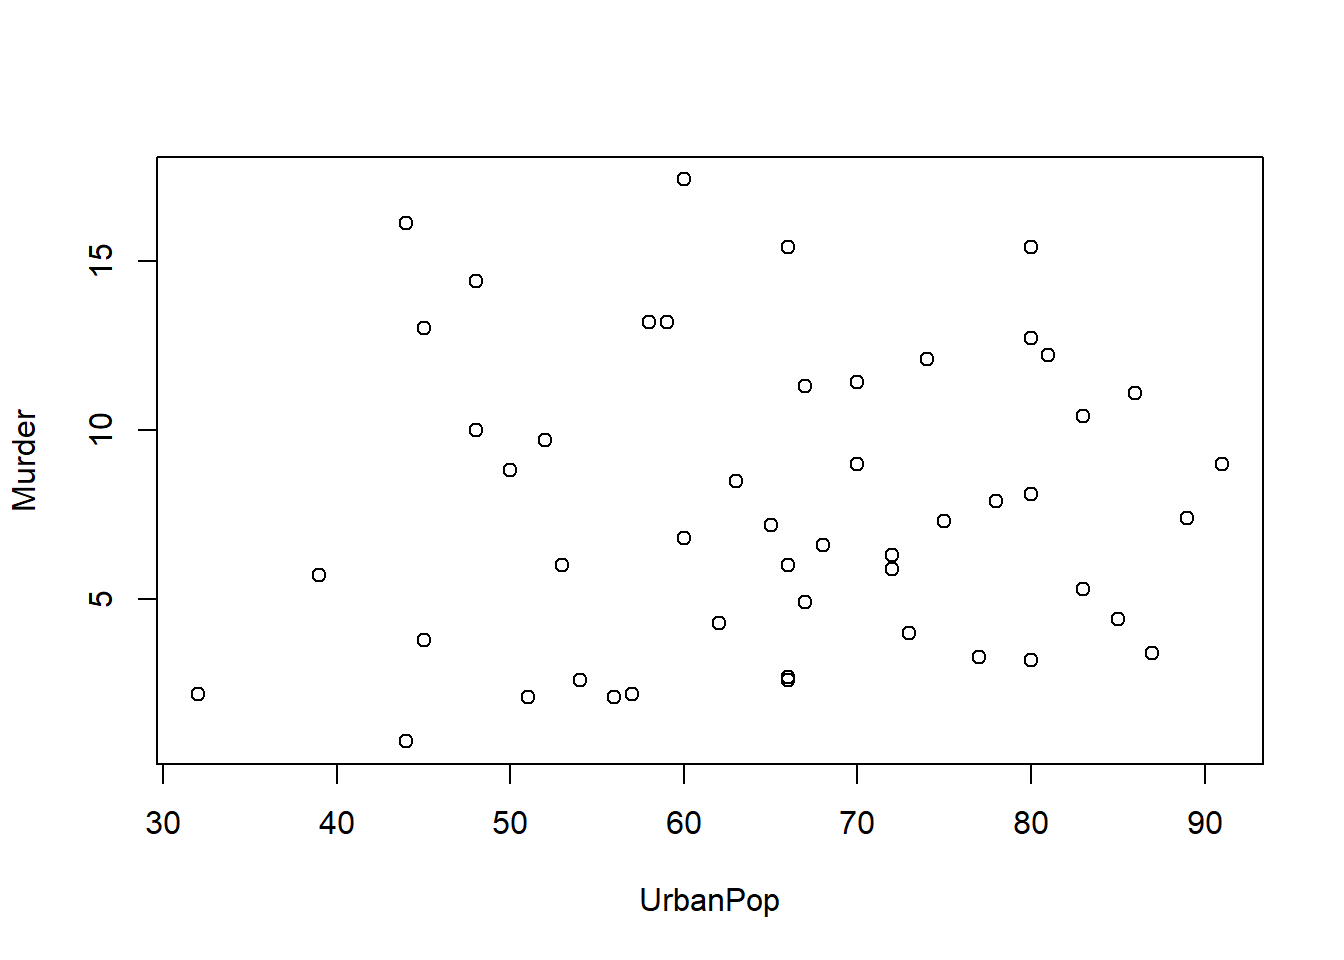
\includegraphics{Completar_Practica_3A_RLogistica_v1_ALUMNOS_files/figure-latex/unnamed-chunk-3-1.pdf}

\begin{Shaded}
\begin{Highlighting}[]
\NormalTok{mydata }\SpecialCharTok{\%\textgreater{}\%}
  \FunctionTok{ggplot}\NormalTok{(}\FunctionTok{aes}\NormalTok{(}\AttributeTok{x =}\NormalTok{ admit, }\AttributeTok{y =}\NormalTok{ gpa)) }\SpecialCharTok{+}
  \FunctionTok{geom\_boxplot}\NormalTok{(}\FunctionTok{aes}\NormalTok{(}\AttributeTok{color =}\NormalTok{ admit))}
\end{Highlighting}
\end{Shaded}

\includegraphics{Completar_Practica_3A_RLogistica_v1_ALUMNOS_files/figure-latex/unnamed-chunk-3-2.pdf}

\begin{Shaded}
\begin{Highlighting}[]
\CommentTok{\#También se podrían haber realizado esos diagramas con:}
\CommentTok{\# boxplot(mydata$gre \textasciitilde{} mydata$admit)}
\CommentTok{\# boxplot(mydata$gpa \textasciitilde{} mydata$admit)}
\end{Highlighting}
\end{Shaded}

\begin{Shaded}
\begin{Highlighting}[]
\CommentTok{\#Ahora separamos los boxplot para cada nivel de la categoria rank}
\NormalTok{mydata }\SpecialCharTok{\%\textgreater{}\%}
  \FunctionTok{ggplot}\NormalTok{(}\FunctionTok{aes}\NormalTok{(}\AttributeTok{x =}\NormalTok{ admit, }\AttributeTok{y =}\NormalTok{ gre)) }\SpecialCharTok{+}
  \FunctionTok{geom\_boxplot}\NormalTok{(}\FunctionTok{aes}\NormalTok{(}\AttributeTok{fill =}\NormalTok{ admit)) }\SpecialCharTok{+}
  \FunctionTok{facet\_grid}\NormalTok{(.}\SpecialCharTok{\textasciitilde{}}\NormalTok{ rank)}
\end{Highlighting}
\end{Shaded}


\includegraphics{Completar_Practica_3A_RLogistica_v1_ALUMNOS_files/figure-latex/unnamed-chunk-4-1.pdf}

\begin{Shaded}
\begin{Highlighting}[]
\NormalTok{mydata }\SpecialCharTok{\%\textgreater{}\%}
  \FunctionTok{ggplot}\NormalTok{(}\FunctionTok{aes}\NormalTok{(}\AttributeTok{x =}\NormalTok{ admit, }\AttributeTok{y =}\NormalTok{ gpa)) }\SpecialCharTok{+}
  \FunctionTok{geom\_boxplot}\NormalTok{(}\FunctionTok{aes}\NormalTok{(}\AttributeTok{fill =}\NormalTok{ admit)) }\SpecialCharTok{+}
  \FunctionTok{facet\_grid}\NormalTok{ (.}\SpecialCharTok{\textasciitilde{}}\NormalTok{ rank)}
\end{Highlighting}
\end{Shaded}

\includegraphics{Completar_Practica_3A_RLogistica_v1_ALUMNOS_files/figure-latex/unnamed-chunk-4-2.pdf}

\begin{Shaded}
\begin{Highlighting}[]
\FunctionTok{ggplot}\NormalTok{(}\AttributeTok{data =}\NormalTok{ mydata, }\FunctionTok{aes}\NormalTok{(}\AttributeTok{x =}\NormalTok{ , }\AttributeTok{y =}\NormalTok{ gre, }\AttributeTok{color =}\NormalTok{ )) }\SpecialCharTok{+}
  \FunctionTok{geom\_boxplot}\NormalTok{()}\SpecialCharTok{+}
  \FunctionTok{theme\_bw}\NormalTok{() }\SpecialCharTok{+}
  \FunctionTok{theme}\NormalTok{(}\AttributeTok{legend.position =} \StringTok{"bottom"}\NormalTok{)}
\end{Highlighting}
\end{Shaded}

\includegraphics{Completar_Practica_3A_RLogistica_v1_ALUMNOS_files/figure-latex/unnamed-chunk-4-3.pdf}

\begin{Shaded}
\begin{Highlighting}[]
\FunctionTok{ggplot}\NormalTok{(}\AttributeTok{data =}\NormalTok{ mydata, }\FunctionTok{aes}\NormalTok{(}\AttributeTok{x =}\NormalTok{ admit, }\AttributeTok{y =}\NormalTok{ gpa, }\AttributeTok{color=}\NormalTok{rank)) }\SpecialCharTok{+}
  \FunctionTok{geom\_boxplot}\NormalTok{()}\SpecialCharTok{+}
  \FunctionTok{theme\_bw}\NormalTok{() }\SpecialCharTok{+}
  \FunctionTok{theme}\NormalTok{(}\AttributeTok{legend.position =} \StringTok{"bottom"}\NormalTok{)}
\end{Highlighting}
\end{Shaded}

\includegraphics{Completar_Practica_3A_RLogistica_v1_ALUMNOS_files/figure-latex/unnamed-chunk-4-4.pdf}
En los gráficos anteriores observamos algunos valores atípicos tanto en
gpa como en gre que merecerían una interpretación más detallada. Por
ejemplo, en el último gráfico tenemos una observación atípica (individuo
de la fila 290) con una nota muy baja en gpa, procedente de un centro
tipo 4 y que no ha sido admitido. También tenemos una observación
atípica (individuo de la fila 373) con una nota muy baja en gpa,
procedente de un centro tipo 1 pero que sí ha sido admitido.

Estos individuos no se detectan como observaciones atípicas si hacemos
la nube de puntos de gre y gpa (distinguiendo los subgrupos admitido y
no admitido), y tampoco se observa correlación entre dichas variables:

\begin{Shaded}
\begin{Highlighting}[]
\FunctionTok{plot}\NormalTok{(mydata}\SpecialCharTok{$}\NormalTok{gpa, mydata}\SpecialCharTok{$}\NormalTok{gre, }\AttributeTok{pch =} \FunctionTok{as.integer}\NormalTok{(mydata}\SpecialCharTok{$}\NormalTok{admit))}
\FunctionTok{legend}\NormalTok{(}\StringTok{\textquotesingle{}bottomright\textquotesingle{}}\NormalTok{, }\AttributeTok{legend=}\FunctionTok{c}\NormalTok{(}\StringTok{\textquotesingle{}0\textquotesingle{}}\NormalTok{,}\StringTok{\textquotesingle{}1\textquotesingle{}}\NormalTok{), }\AttributeTok{pch=}\DecValTok{1}\SpecialCharTok{:}\DecValTok{2}\NormalTok{)}
\end{Highlighting}
\end{Shaded}

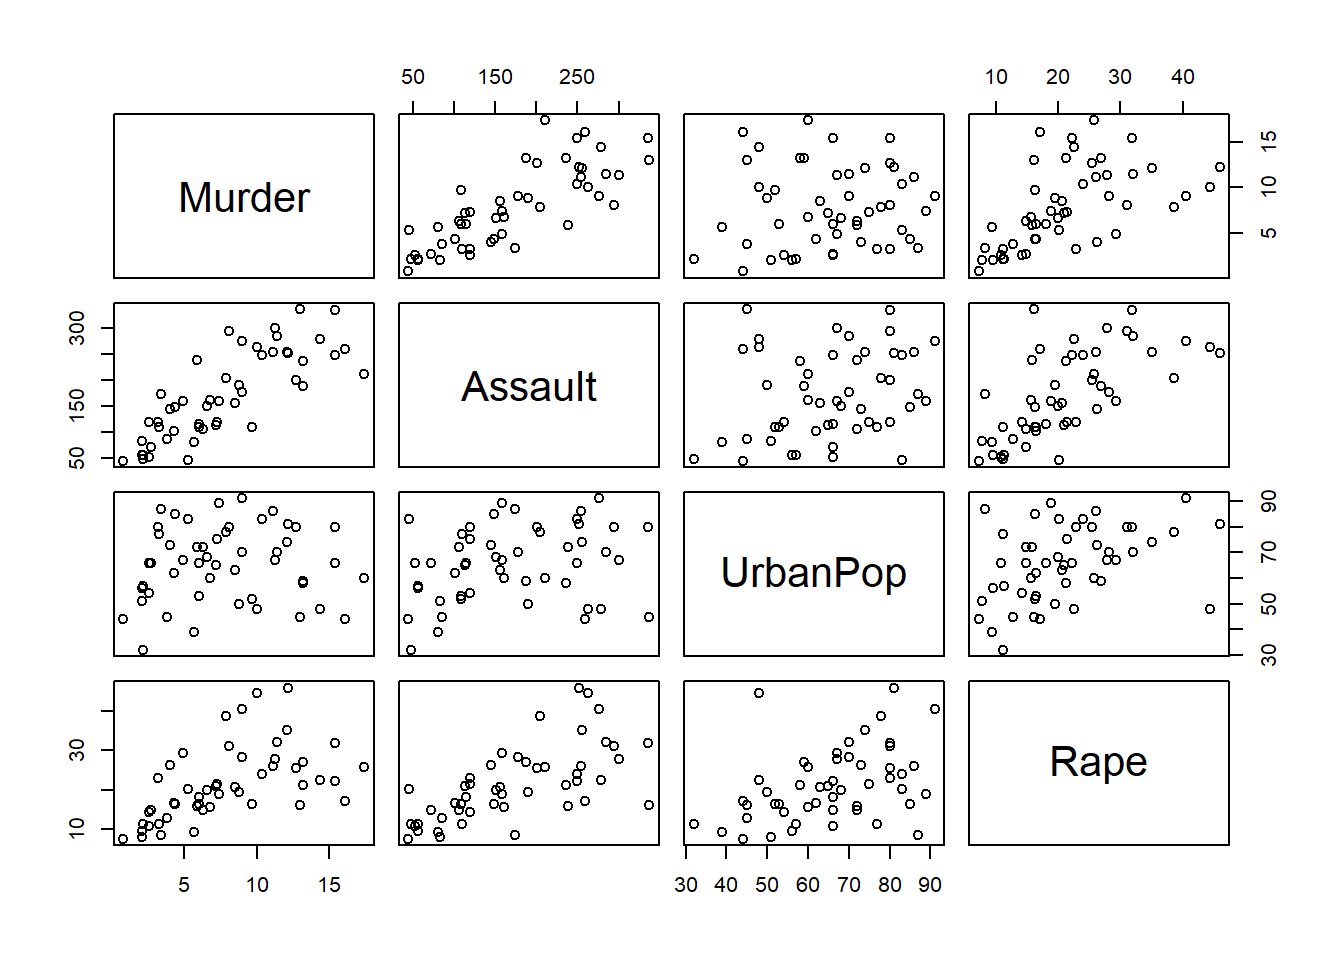
\includegraphics{Completar_Practica_3A_RLogistica_v1_ALUMNOS_files/figure-latex/unnamed-chunk-5-1.pdf}

Ahora vamos a comprobar que no hay celdas vacías (o frecuencias muy
bajas) en las tablas de contingencia de los predictores categóricos y la
variable respuesta. Si hay celdas vacías o con pocos casos, el modelo
RLogistica puede ser inestable y poco fiable.

\begin{Shaded}
\begin{Highlighting}[]
\FunctionTok{addmargins}\NormalTok{(}\FunctionTok{table}\NormalTok{(mydata}\SpecialCharTok{$}\NormalTok{admit, mydata}\SpecialCharTok{$}\NormalTok{rank, }
                 \AttributeTok{dnn =} \FunctionTok{c}\NormalTok{(}\StringTok{"admit"}\NormalTok{, }\StringTok{"rank"}\NormalTok{)))}
\end{Highlighting}
\end{Shaded}

\begin{verbatim}
##      rank
## admit   1   2   3   4 Sum
##   0    28  97  93  55 273
##   1    33  54  28  12 127
##   Sum  61 151 121  67 400
\end{verbatim}

Tras el estudio descriptivo previo, podemos observar en los gráficos que
la tendencia central (mediana) de las puntuaciones en \texttt{gre} y
\texttt{gpa} son más altas para los alumnos admitidos en la universidad
que para los no admitidos. Y mirando la tabla de contingencia anterior,
observamos que la tasa de admitidos frente a no admitidos es mayor para
los centros educativos de procedencia con más prestigio
(\texttt{rank\ =\ 1}).

\hypertarget{estimaciuxf3n-de-los-paruxe1metros-del-modelo-rlogistica-y-muxe9todos-de-selecciuxf3n-de-regresores}{%
\section{2. Estimación de los parámetros del modelo RLogistica y métodos
de selección de
regresores}\label{estimaciuxf3n-de-los-paruxe1metros-del-modelo-rlogistica-y-muxe9todos-de-selecciuxf3n-de-regresores}}

Recordemos que el modelo teórico de Regresión Logística para estos datos
viene dado por:

\[
\log\left(\frac{p}{1-p} \right) =\theta_0+\theta_1 \cdot gre+\theta_2 \cdot gpa+\theta_3 \cdot rank2+\theta_4 \cdot rank3+\theta_5 \cdot rank4\, ,
\] siendo \(p=\Pr(Y=1)\).

Hay que entender las variables \texttt{rank2}, \texttt{rank3} y
\texttt{rank4} como variables binarias (\emph{dummy}) que toman el valor
1 si el valor de \texttt{rank} se corresponde con su índice y valen cero
en caso contrario. Por ejemplo, si \(rank=3\), entonces \(rank2=0\),
\(rank3=1\) y \(rank4=0\).

Estimamos el modelo logístico usando todos los predictores. Para ello,
usamos la función \emph{glm()} de R que sirve para estimar los modelos
lineales generalizados. En particular, el modelo logístico requiere
poner el argumento \texttt{family\ =\ "binomial"} que lleva por defecto
a la función logística como función \texttt{link}.

\begin{Shaded}
\begin{Highlighting}[]
\NormalTok{mylogit }\OtherTok{\textless{}{-}} \FunctionTok{glm}\NormalTok{(admit }\SpecialCharTok{\textasciitilde{}}\NormalTok{ gre }\SpecialCharTok{+}\NormalTok{ gpa }\SpecialCharTok{+}\NormalTok{ rank, }\AttributeTok{data =}\NormalTok{ mydata, }\AttributeTok{family =} \StringTok{"binomial"}\NormalTok{)}
\FunctionTok{summary}\NormalTok{(mylogit)}
\end{Highlighting}
\end{Shaded}

\begin{verbatim}
## 
## Call:
## glm(formula = admit ~ gre + gpa + rank, family = "binomial", 
##     data = mydata)
## 
## Coefficients:
##              Estimate Std. Error z value Pr(>|z|)    
## (Intercept) -3.989979   1.139951  -3.500 0.000465 ***
## gre          0.002264   0.001094   2.070 0.038465 *  
## gpa          0.804038   0.331819   2.423 0.015388 *  
## rank2       -0.675443   0.316490  -2.134 0.032829 *  
## rank3       -1.340204   0.345306  -3.881 0.000104 ***
## rank4       -1.551464   0.417832  -3.713 0.000205 ***
## ---
## Signif. codes:  0 '***' 0.001 '**' 0.01 '*' 0.05 '.' 0.1 ' ' 1
## 
## (Dispersion parameter for binomial family taken to be 1)
## 
##     Null deviance: 499.98  on 399  degrees of freedom
## Residual deviance: 458.52  on 394  degrees of freedom
## AIC: 470.52
## 
## Number of Fisher Scoring iterations: 4
\end{verbatim}

De los resultados anteriores, obtenemos que el modelo lineal ajustado
(que explica el logaritmo de los \emph{odds}) viene dado por:

\[
-3.989979+0.002264\cdot gre+0.804038\cdot gpa-0.675443\cdot rank2-1.340204\cdot rank3-1.551464\cdot rank4
\]

La \textbf{interpretación de los coefientes} del modelo RLogistica sería
la siguiente:

Por cada unidad adicional en la variable \texttt{gre}, el logaritmo de
los \emph{odds} de admitido frente a no admitido aumenta en 0.002264.

Por cada unidad adicional en la variable \texttt{gpa}, el logaritmo de
los \emph{odds} de admitido frente a no admitido aumenta en 0.804038.

Haber asistido a un centro educativo con prestigio 2 frente a prestigio
1, produce un cambio en el logaritmo de los \emph{odds} de -0.675443, es
decir, el logaritmo de los \emph{odds} de admitido frente a no admitido
disminuye en 0.675443.

Además de la estimación de los coeficientes de regresión, obtenemos sus
p-valores correspondientes. Observamos que en este caso son todos
significativos (inferiores a 0.05), lo que nos hace sospechar que el
modelo no va a ser reducible.

Como en el caso de RLM, podemos aplicar los \textbf{métodos de selección
de regresores} \emph{backward}, \emph{fordward} y \emph{stepwise}, para
ver si el modelo completo es reducible a otro más sencillo (con menos
predictores).

\begin{Shaded}
\begin{Highlighting}[]
\NormalTok{modelo\_backward }\OtherTok{\textless{}{-}} \FunctionTok{step}\NormalTok{(mylogit, }\AttributeTok{direction =} \StringTok{"backward"}\NormalTok{)}
\end{Highlighting}
\end{Shaded}

\begin{verbatim}
## Start:  AIC=470.52
## admit ~ gre + gpa + rank
## 
##        Df Deviance    AIC
## <none>      458.52 470.52
## - gre   1   462.88 472.88
## - gpa   1   464.53 474.53
## - rank  3   480.34 486.34
\end{verbatim}

Los resultados anteriores indican que el modelo no es reducible. Se
obtienen resultados similares con los otros métodos, como mostramos a
continuación.

\begin{Shaded}
\begin{Highlighting}[]
\NormalTok{modelo\_nulo }\OtherTok{\textless{}{-}} \FunctionTok{glm}\NormalTok{(admit }\SpecialCharTok{\textasciitilde{}} \DecValTok{1}\NormalTok{, }\AttributeTok{data =}\NormalTok{ mydata, }\AttributeTok{family =} \StringTok{"binomial"}\NormalTok{)}
\NormalTok{modelo\_forward }\OtherTok{\textless{}{-}} \FunctionTok{step}\NormalTok{(modelo\_nulo, }\AttributeTok{scope =} \FunctionTok{formula}\NormalTok{(mylogit), }\AttributeTok{direction =} \StringTok{"forward"}\NormalTok{)}
\end{Highlighting}
\end{Shaded}

\begin{verbatim}
## Start:  AIC=501.98
## admit ~ 1
## 
##        Df Deviance    AIC
## + rank  3   474.97 482.97
## + gre   1   486.06 490.06
## + gpa   1   486.97 490.97
## <none>      499.98 501.98
## 
## Step:  AIC=482.97
## admit ~ rank
## 
##        Df Deviance    AIC
## + gpa   1   462.88 472.88
## + gre   1   464.53 474.53
## <none>      474.97 482.97
## 
## Step:  AIC=472.88
## admit ~ rank + gpa
## 
##        Df Deviance    AIC
## + gre   1   458.52 470.52
## <none>      462.88 472.88
## 
## Step:  AIC=470.52
## admit ~ rank + gpa + gre
\end{verbatim}

\begin{Shaded}
\begin{Highlighting}[]
\NormalTok{modelo\_stepwise }\OtherTok{\textless{}{-}} \FunctionTok{step}\NormalTok{(modelo\_nulo, }\AttributeTok{scope =} \FunctionTok{formula}\NormalTok{(mylogit), }\AttributeTok{direction =} \StringTok{"both"}\NormalTok{)}
\end{Highlighting}
\end{Shaded}

\begin{verbatim}
## Start:  AIC=501.98
## admit ~ 1
## 
##        Df Deviance    AIC
## + rank  3   474.97 482.97
## + gre   1   486.06 490.06
## + gpa   1   486.97 490.97
## <none>      499.98 501.98
## 
## Step:  AIC=482.97
## admit ~ rank
## 
##        Df Deviance    AIC
## + gpa   1   462.88 472.88
## + gre   1   464.53 474.53
## <none>      474.97 482.97
## - rank  3   499.98 501.98
## 
## Step:  AIC=472.88
## admit ~ rank + gpa
## 
##        Df Deviance    AIC
## + gre   1   458.52 470.52
## <none>      462.88 472.88
## - gpa   1   474.97 482.97
## - rank  3   486.97 490.97
## 
## Step:  AIC=470.52
## admit ~ rank + gpa + gre
## 
##        Df Deviance    AIC
## <none>      458.52 470.52
## - gre   1   462.88 472.88
## - gpa   1   464.53 474.53
## - rank  3   480.34 486.34
\end{verbatim}

Observamos que los tres métodos conducen al modelo completo con los 3
predictores, así que ese será nuestro modelo de referencia.

La selección del modelo también puede realizarse con la función
\emph{stepAIC()} del paquete \texttt{MASS}, obteniendo los mismos
resultados que en el caso anterior.

\begin{Shaded}
\begin{Highlighting}[]
\CommentTok{\# library("MASS")}
\CommentTok{\# modelo\_backward2 \textless{}{-} stepAIC(mylogit, direction = "backward")}
\CommentTok{\# modelo\_forward2 \textless{}{-} stepAIC(modelo\_nulo, scope = formula(mylogit), direction = "forward")}
\CommentTok{\# modelo\_stepwise2 \textless{}{-} stepAIC(modelo\_nulo, scope = formula(mylogit), direction = "both")}
\end{Highlighting}
\end{Shaded}

La \textbf{bondad del ajuste} del modelo se puede medir a través del
\texttt{AIC} (criterio de Akaike), siendo mejor el ajuste cuanto menor
sea el AIC. También se puede usar la \texttt{devianza\ residual}, siendo
mejor el ajuste cuanto menor sea la \texttt{devianza}.

\begin{Shaded}
\begin{Highlighting}[]
\NormalTok{mylogit}\SpecialCharTok{$}\NormalTok{aic }\CommentTok{\#Valor AIC del modelo}
\end{Highlighting}
\end{Shaded}

\begin{verbatim}
## [1] 470.5175
\end{verbatim}

\begin{Shaded}
\begin{Highlighting}[]
\NormalTok{mylogit}\SpecialCharTok{$}\NormalTok{deviance }\CommentTok{\#Valor de la devianza }
\end{Highlighting}
\end{Shaded}

\begin{verbatim}
## [1] 458.5175
\end{verbatim}

\begin{Shaded}
\begin{Highlighting}[]
\CommentTok{\#Comprobamos que la devianza del modelo coincide con {-}2*log(likelihood)}
\SpecialCharTok{{-}}\DecValTok{2}\SpecialCharTok{*}\FunctionTok{logLik}\NormalTok{(mylogit) }
\end{Highlighting}
\end{Shaded}

\begin{verbatim}
## 'log Lik.' 458.5175 (df=6)
\end{verbatim}

\hypertarget{inferencias-en-el-modelo-rlogistica.-predicciones}{%
\section{3. Inferencias en el modelo RLogistica.
Predicciones}\label{inferencias-en-el-modelo-rlogistica.-predicciones}}

Una vez validado el modelo RLogistica, lo cual se realizará en una
sección posterior, tenemos garantías para realizar inferencias con dicho
modelo. Estas inferencias incluyen la obtención de intervalos de
confianza para los parámetros de regresión, la prueba de significación
del modelo, pruebas individuales de significación de los predictores y
también para un conjunto de predictores (test de Wald).

En primer lugar calculamos los \textbf{intervalos de confianza} para los
parámetros de regresión.

\begin{Shaded}
\begin{Highlighting}[]
\FunctionTok{confint}\NormalTok{(mylogit, }\AttributeTok{level =} \FloatTok{0.95}\NormalTok{)}
\end{Highlighting}
\end{Shaded}

\begin{verbatim}
## Waiting for profiling to be done...
\end{verbatim}

\begin{verbatim}
##                     2.5 %       97.5 %
## (Intercept) -6.2716202334 -1.792547080
## gre          0.0001375921  0.004435874
## gpa          0.1602959439  1.464142727
## rank2       -1.3008888002 -0.056745722
## rank3       -2.0276713127 -0.670372346
## rank4       -2.4000265384 -0.753542605
\end{verbatim}

Recordemos que los coeficientes del modelo miden la variación del
logaritmo de los \emph{odds} por unidad de cambio en el correspondiente
predictor. Tomando exponenciales sobre los coeficientes y sobre los
extremos del intervalo de confianza, medimos las variaciones producidas
sobre los \emph{odds} directamente (sin tomar logaritmo).

\begin{Shaded}
\begin{Highlighting}[]
\DocumentationTok{\#\# odds ratios}
\FunctionTok{exp}\NormalTok{(}\FunctionTok{coef}\NormalTok{(mylogit))}
\end{Highlighting}
\end{Shaded}

\begin{verbatim}
## (Intercept)         gre         gpa       rank2       rank3       rank4 
##   0.0185001   1.0022670   2.2345448   0.5089310   0.2617923   0.2119375
\end{verbatim}

\begin{Shaded}
\begin{Highlighting}[]
\DocumentationTok{\#\# odds ratios con sus Intervalos de Confianza}
\FunctionTok{exp}\NormalTok{(}\FunctionTok{cbind}\NormalTok{(}\AttributeTok{OR =} \FunctionTok{coef}\NormalTok{(mylogit), }\FunctionTok{confint}\NormalTok{(mylogit, }\AttributeTok{level =} \FloatTok{0.95}\NormalTok{)))}
\end{Highlighting}
\end{Shaded}

\begin{verbatim}
## Waiting for profiling to be done...
\end{verbatim}

\begin{verbatim}
##                    OR       2.5 %    97.5 %
## (Intercept) 0.0185001 0.001889165 0.1665354
## gre         1.0022670 1.000137602 1.0044457
## gpa         2.2345448 1.173858216 4.3238349
## rank2       0.5089310 0.272289674 0.9448343
## rank3       0.2617923 0.131641717 0.5115181
## rank4       0.2119375 0.090715546 0.4706961
\end{verbatim}

Medimos la \textbf{significación del modelo} comparando la devianza del
modelo completo frente a la devianza del modelo nulo. Esta diferencia
sigue una Chi-cuadrado con los grados de libertad dados por la
diferencia de grados de ambos modelos.

\begin{Shaded}
\begin{Highlighting}[]
\NormalTok{diferencia\_devianzas }\OtherTok{\textless{}{-}}\NormalTok{ mylogit}\SpecialCharTok{$}\NormalTok{null.deviance }\SpecialCharTok{{-}}\NormalTok{ mylogit}\SpecialCharTok{$}\NormalTok{deviance}
\NormalTok{grados\_libertad }\OtherTok{\textless{}{-}}\NormalTok{ mylogit}\SpecialCharTok{$}\NormalTok{df.null }\SpecialCharTok{{-}}\NormalTok{ mylogit}\SpecialCharTok{$}\NormalTok{df.residual}
\NormalTok{p\_valor }\OtherTok{\textless{}{-}} \FunctionTok{pchisq}\NormalTok{(diferencia\_devianzas, }\AttributeTok{df =}\NormalTok{ grados\_libertad, }\AttributeTok{lower.tail =} \ConstantTok{FALSE}\NormalTok{)}
\NormalTok{p\_valor}
\end{Highlighting}
\end{Shaded}

\begin{verbatim}
## [1] 7.578194e-08
\end{verbatim}

Obsérvese que el p-valor resultante permite concluir que el modelo
completo es significativo.

La signficación individual de cada predictor se obtiene con el test de
Wald y el estadístico \texttt{Z}, que aparecen directamente al hacer el
\texttt{summary} del modelo (véase más arriba, donde se indicó que en
este caso todos los predictores resultan significativos
individualmente).

Podemos hacer un estudio de la significacióm conjunta de la variable
\texttt{rank}, pues se trata de un factor con 4 niveles que da lugar a 3
predictores (en el resumen del modelo se puede ver que
\texttt{rank\ =\ 1} es el nivel de referencia). Para ello, podemos usar
la función \emph{wald.este()} del paquete \texttt{aod}.

\begin{Shaded}
\begin{Highlighting}[]
\FunctionTok{library}\NormalTok{(}\StringTok{"aod"}\NormalTok{)}
\FunctionTok{wald.test}\NormalTok{(}\AttributeTok{b =} \FunctionTok{coef}\NormalTok{(mylogit), }\AttributeTok{Sigma =} \FunctionTok{vcov}\NormalTok{(mylogit), }\AttributeTok{Terms =} \DecValTok{4}\SpecialCharTok{:}\DecValTok{6}\NormalTok{) }
\end{Highlighting}
\end{Shaded}

\begin{verbatim}
## Wald test:
## ----------
## 
## Chi-squared test:
## X2 = 20.9, df = 3, P(> X2) = 0.00011
\end{verbatim}

\begin{Shaded}
\begin{Highlighting}[]
\CommentTok{\#Observar que los términos 4, 5 y 6 del resumen del modelo son }
\CommentTok{\#los correspondientes a rank2, rank3 y rank4}
\end{Highlighting}
\end{Shaded}

Obsérvese que el p-valor resultante permite concluir que la variable
``rank'' es significativa.

También podemos comparar si hay diferencia entre los coeficientes de dos
niveles de \texttt{rank}. Por ejemplo, comparamos si hay diferencia
entre los coeficientes de los niveles 2 y 3 de \texttt{rank} de la
siguiente manera. Hay que tener en cuenta el orden de los parámetros de
regresión en el modelo logit, que como muestra la salida del modelo son
los correspondientes a la constante, gre, gpa, rank2, rank3 y rank4. Por
tanto, la combinación (0,0,0,1,-1,0) se refiere al contraste de igualdad
entre los coeficientes de rank2 y rank3:

\begin{Shaded}
\begin{Highlighting}[]
\NormalTok{combinacion }\OtherTok{\textless{}{-}} \FunctionTok{cbind}\NormalTok{(}\DecValTok{0}\NormalTok{, }\DecValTok{0}\NormalTok{, }\DecValTok{0}\NormalTok{, }\DecValTok{1}\NormalTok{, }\SpecialCharTok{{-}}\DecValTok{1}\NormalTok{, }\DecValTok{0}\NormalTok{)}
\FunctionTok{wald.test}\NormalTok{(}\AttributeTok{b =} \FunctionTok{coef}\NormalTok{(mylogit), }\AttributeTok{Sigma =} \FunctionTok{vcov}\NormalTok{(mylogit), }\AttributeTok{L =}\NormalTok{ combinacion)}
\end{Highlighting}
\end{Shaded}

\begin{verbatim}
## Wald test:
## ----------
## 
## Chi-squared test:
## X2 = 5.5, df = 1, P(> X2) = 0.019
\end{verbatim}

Obsérvese que el p-valor resultante permite concluir que hay diferencia
significativa entre los coeficientes de \texttt{rank\ =\ 2} y
\texttt{rank\ =\ 3}.

Para realizar \textbf{predicciones} del modelo RLogistica, usamos la
función \emph{predict()}, que en este caso permite hacer predicciones de
la variable respuesta (argumento \texttt{type\ =\ "response"}) o del
modelo lineal ajustado (argumento por defecto,
\texttt{type\ =\ "link"}).

Por ejemplo, hagamos la predicción para un alumno con
\texttt{gre\ =\ 750}, \texttt{gpa\ =\ 3.5} y \texttt{rank\ =\ 2}.

\begin{Shaded}
\begin{Highlighting}[]
\NormalTok{nuevos\_1 }\OtherTok{\textless{}{-}} \FunctionTok{data.frame}\NormalTok{(}\AttributeTok{gre =} \DecValTok{750}\NormalTok{, }\AttributeTok{gpa =} \FloatTok{3.5}\NormalTok{, }\AttributeTok{rank =} \FunctionTok{as.factor}\NormalTok{(}\DecValTok{2}\NormalTok{))}
\FunctionTok{predict}\NormalTok{(mylogit , }\AttributeTok{newdata =}\NormalTok{ nuevos\_1, }\AttributeTok{type =} \StringTok{"link"}\NormalTok{)}
\end{Highlighting}
\end{Shaded}

\begin{verbatim}
##          1 
## -0.1529712
\end{verbatim}

\begin{Shaded}
\begin{Highlighting}[]
\FunctionTok{predict}\NormalTok{(mylogit , }\AttributeTok{newdata =}\NormalTok{ nuevos\_1, }\AttributeTok{type =} \StringTok{"response"}\NormalTok{)}
\end{Highlighting}
\end{Shaded}

\begin{verbatim}
##         1 
## 0.4618316
\end{verbatim}

Es decir, la predicción indica que para un alumno de esas
características, la probabilidad de ser admitido es
\(p=\Pr(Y=1)=0.4618316\). Podemos comprobar el logaritmo de los odds en
este caso sería log(p/(1-p))=-0.1529712.

Si queremos ver el efecto del prestigio del centro de procedencia en la
admisión, podemos fijar \texttt{gre} y \texttt{gpa} en sus valores
medios y variar \texttt{rank}.

\begin{Shaded}
\begin{Highlighting}[]
\NormalTok{nuevos\_2 }\OtherTok{\textless{}{-}} \FunctionTok{with}\NormalTok{(mydata, }\FunctionTok{data.frame}\NormalTok{(}\AttributeTok{gre =} \FunctionTok{mean}\NormalTok{(gre), }\AttributeTok{gpa =} \FunctionTok{mean}\NormalTok{(gpa), }\AttributeTok{rank =} \FunctionTok{factor}\NormalTok{(}\DecValTok{1}\SpecialCharTok{:}\DecValTok{4}\NormalTok{)))}
\NormalTok{nuevos\_2}\SpecialCharTok{$}\NormalTok{rank\_predic }\OtherTok{\textless{}{-}} \FunctionTok{predict}\NormalTok{(mylogit, }\AttributeTok{newdata =}\NormalTok{ nuevos\_2, }\AttributeTok{type =} \StringTok{"response"}\NormalTok{)}
\NormalTok{nuevos\_2}
\end{Highlighting}
\end{Shaded}

\begin{verbatim}
##     gre    gpa rank rank_predic
## 1 587.7 3.3899    1   0.5166016
## 2 587.7 3.3899    2   0.3522846
## 3 587.7 3.3899    3   0.2186120
## 4 587.7 3.3899    4   0.1846684
\end{verbatim}

De esta forma comprobamos como la variable \texttt{rank} es muy
relevante sobre la admisión. Por ejemplo, para un alumno con los valores
medios de \texttt{gre} y \texttt{gpa}, el modelo logit indica que el
alumno será admitido si rank=1 (probabilidad superior a 0.5) y no será
admitido en los otros casos (probabilidades inferiores a 0.5).

Ahora fijamos \texttt{gpa} en su media, movemos \texttt{rank} en sus 4
niveles y hacemos un grid con el predictor \texttt{gre}. Así vemos el
efecto de la nota del examen de acceso (predictor \texttt{gre}) en la
admisión.

\begin{Shaded}
\begin{Highlighting}[]
\NormalTok{nuevos\_3 }\OtherTok{\textless{}{-}} \FunctionTok{with}\NormalTok{(mydata, }
                 \FunctionTok{data.frame}\NormalTok{(}\AttributeTok{gre =} \FunctionTok{rep}\NormalTok{(}\FunctionTok{seq}\NormalTok{(}\AttributeTok{from =} \DecValTok{200}\NormalTok{, }\AttributeTok{to =} \DecValTok{800}\NormalTok{, }\AttributeTok{length.out =} \DecValTok{100}\NormalTok{),}
                                      \DecValTok{4}\NormalTok{), }
                            \AttributeTok{gpa =} \FunctionTok{mean}\NormalTok{(gpa), }
                            \AttributeTok{rank =} \FunctionTok{factor}\NormalTok{(}\FunctionTok{rep}\NormalTok{(}\DecValTok{1}\SpecialCharTok{:}\DecValTok{4}\NormalTok{, }\AttributeTok{each =} \DecValTok{100}\NormalTok{))))}

\NormalTok{nuevos\_3}\SpecialCharTok{$}\NormalTok{gre\_predic }\OtherTok{\textless{}{-}} \FunctionTok{predict}\NormalTok{(mylogit, }\AttributeTok{newdata =}\NormalTok{ nuevos\_3, }\AttributeTok{type =} \StringTok{"response"}\NormalTok{)}
\NormalTok{nuevos\_3}
\end{Highlighting}
\end{Shaded}

\begin{verbatim}
##          gre    gpa rank gre_predic
## 1   200.0000 3.3899    1 0.30757371
## 2   206.0606 3.3899    1 0.31050419
## 3   212.1212 3.3899    1 0.31344995
## 4   218.1818 3.3899    1 0.31641083
## 5   224.2424 3.3899    1 0.31938667
## 6   230.3030 3.3899    1 0.32237730
## 7   236.3636 3.3899    1 0.32538254
## 8   242.4242 3.3899    1 0.32840222
## 9   248.4848 3.3899    1 0.33143616
## 10  254.5455 3.3899    1 0.33448416
## 11  260.6061 3.3899    1 0.33754605
## 12  266.6667 3.3899    1 0.34062162
## 13  272.7273 3.3899    1 0.34371067
## 14  278.7879 3.3899    1 0.34681300
## 15  284.8485 3.3899    1 0.34992840
## 16  290.9091 3.3899    1 0.35305667
## 17  296.9697 3.3899    1 0.35619757
## 18  303.0303 3.3899    1 0.35935090
## 19  309.0909 3.3899    1 0.36251642
## 20  315.1515 3.3899    1 0.36569391
## 21  321.2121 3.3899    1 0.36888313
## 22  327.2727 3.3899    1 0.37208386
## 23  333.3333 3.3899    1 0.37529584
## 24  339.3939 3.3899    1 0.37851883
## 25  345.4545 3.3899    1 0.38175259
## 26  351.5152 3.3899    1 0.38499686
## 27  357.5758 3.3899    1 0.38825138
## 28  363.6364 3.3899    1 0.39151591
## 29  369.6970 3.3899    1 0.39479017
## 30  375.7576 3.3899    1 0.39807389
## 31  381.8182 3.3899    1 0.40136682
## 32  387.8788 3.3899    1 0.40466867
## 33  393.9394 3.3899    1 0.40797918
## 34  400.0000 3.3899    1 0.41129806
## 35  406.0606 3.3899    1 0.41462502
## 36  412.1212 3.3899    1 0.41795979
## 37  418.1818 3.3899    1 0.42130208
## 38  424.2424 3.3899    1 0.42465160
## 39  430.3030 3.3899    1 0.42800805
## 40  436.3636 3.3899    1 0.43137114
## 41  442.4242 3.3899    1 0.43474057
## 42  448.4848 3.3899    1 0.43811604
## 43  454.5455 3.3899    1 0.44149725
## 44  460.6061 3.3899    1 0.44488390
## 45  466.6667 3.3899    1 0.44827567
## 46  472.7273 3.3899    1 0.45167226
## 47  478.7879 3.3899    1 0.45507335
## 48  484.8485 3.3899    1 0.45847865
## 49  490.9091 3.3899    1 0.46188783
## 50  496.9697 3.3899    1 0.46530057
## 51  503.0303 3.3899    1 0.46871657
## 52  509.0909 3.3899    1 0.47213550
## 53  515.1515 3.3899    1 0.47555705
## 54  521.2121 3.3899    1 0.47898089
## 55  527.2727 3.3899    1 0.48240671
## 56  533.3333 3.3899    1 0.48583418
## 57  539.3939 3.3899    1 0.48926299
## 58  545.4545 3.3899    1 0.49269281
## 59  551.5152 3.3899    1 0.49612331
## 60  557.5758 3.3899    1 0.49955418
## 61  563.6364 3.3899    1 0.50298510
## 62  569.6970 3.3899    1 0.50641573
## 63  575.7576 3.3899    1 0.50984576
## 64  581.8182 3.3899    1 0.51327486
## 65  587.8788 3.3899    1 0.51670271
## 66  593.9394 3.3899    1 0.52012899
## 67  600.0000 3.3899    1 0.52355338
## 68  606.0606 3.3899    1 0.52697555
## 69  612.1212 3.3899    1 0.53039519
## 70  618.1818 3.3899    1 0.53381198
## 71  624.2424 3.3899    1 0.53722560
## 72  630.3030 3.3899    1 0.54063574
## 73  636.3636 3.3899    1 0.54404207
## 74  642.4242 3.3899    1 0.54744429
## 75  648.4848 3.3899    1 0.55084208
## 76  654.5455 3.3899    1 0.55423513
## 77  660.6061 3.3899    1 0.55762314
## 78  666.6667 3.3899    1 0.56100579
## 79  672.7273 3.3899    1 0.56438278
## 80  678.7879 3.3899    1 0.56775381
## 81  684.8485 3.3899    1 0.57111858
## 82  690.9091 3.3899    1 0.57447678
## 83  696.9697 3.3899    1 0.57782813
## 84  703.0303 3.3899    1 0.58117233
## 85  709.0909 3.3899    1 0.58450908
## 86  715.1515 3.3899    1 0.58783810
## 87  721.2121 3.3899    1 0.59115911
## 88  727.2727 3.3899    1 0.59447182
## 89  733.3333 3.3899    1 0.59777594
## 90  739.3939 3.3899    1 0.60107122
## 91  745.4545 3.3899    1 0.60435736
## 92  751.5152 3.3899    1 0.60763411
## 93  757.5758 3.3899    1 0.61090119
## 94  763.6364 3.3899    1 0.61415834
## 95  769.6970 3.3899    1 0.61740530
## 96  775.7576 3.3899    1 0.62064181
## 97  781.8182 3.3899    1 0.62386763
## 98  787.8788 3.3899    1 0.62708249
## 99  793.9394 3.3899    1 0.63028616
## 100 800.0000 3.3899    1 0.63347840
## 101 200.0000 3.3899    2 0.18438297
## 102 206.0606 3.3899    2 0.18645578
## 103 212.1212 3.3899    2 0.18854651
## 104 218.1818 3.3899    2 0.19065518
## 105 224.2424 3.3899    2 0.19278184
## 106 230.3030 3.3899    2 0.19492650
## 107 236.3636 3.3899    2 0.19708920
## 108 242.4242 3.3899    2 0.19926995
## 109 248.4848 3.3899    2 0.20146878
## 110 254.5455 3.3899    2 0.20368570
## 111 260.6061 3.3899    2 0.20592073
## 112 266.6667 3.3899    2 0.20817386
## 113 272.7273 3.3899    2 0.21044512
## 114 278.7879 3.3899    2 0.21273450
## 115 284.8485 3.3899    2 0.21504200
## 116 290.9091 3.3899    2 0.21736762
## 117 296.9697 3.3899    2 0.21971135
## 118 303.0303 3.3899    2 0.22207318
## 119 309.0909 3.3899    2 0.22445310
## 120 315.1515 3.3899    2 0.22685108
## 121 321.2121 3.3899    2 0.22926711
## 122 327.2727 3.3899    2 0.23170116
## 123 333.3333 3.3899    2 0.23415321
## 124 339.3939 3.3899    2 0.23662320
## 125 345.4545 3.3899    2 0.23911112
## 126 351.5152 3.3899    2 0.24161692
## 127 357.5758 3.3899    2 0.24414055
## 128 363.6364 3.3899    2 0.24668197
## 129 369.6970 3.3899    2 0.24924112
## 130 375.7576 3.3899    2 0.25181794
## 131 381.8182 3.3899    2 0.25441238
## 132 387.8788 3.3899    2 0.25702436
## 133 393.9394 3.3899    2 0.25965382
## 134 400.0000 3.3899    2 0.26230069
## 135 406.0606 3.3899    2 0.26496488
## 136 412.1212 3.3899    2 0.26764631
## 137 418.1818 3.3899    2 0.27034490
## 138 424.2424 3.3899    2 0.27306055
## 139 430.3030 3.3899    2 0.27579317
## 140 436.3636 3.3899    2 0.27854266
## 141 442.4242 3.3899    2 0.28130891
## 142 448.4848 3.3899    2 0.28409181
## 143 454.5455 3.3899    2 0.28689126
## 144 460.6061 3.3899    2 0.28970713
## 145 466.6667 3.3899    2 0.29253930
## 146 472.7273 3.3899    2 0.29538764
## 147 478.7879 3.3899    2 0.29825202
## 148 484.8485 3.3899    2 0.30113231
## 149 490.9091 3.3899    2 0.30402836
## 150 496.9697 3.3899    2 0.30694004
## 151 503.0303 3.3899    2 0.30986718
## 152 509.0909 3.3899    2 0.31280964
## 153 515.1515 3.3899    2 0.31576725
## 154 521.2121 3.3899    2 0.31873986
## 155 527.2727 3.3899    2 0.32172729
## 156 533.3333 3.3899    2 0.32472938
## 157 539.3939 3.3899    2 0.32774595
## 158 545.4545 3.3899    2 0.33077681
## 159 551.5152 3.3899    2 0.33382178
## 160 557.5758 3.3899    2 0.33688067
## 161 563.6364 3.3899    2 0.33995329
## 162 569.6970 3.3899    2 0.34303943
## 163 575.7576 3.3899    2 0.34613890
## 164 581.8182 3.3899    2 0.34925148
## 165 587.8788 3.3899    2 0.35237697
## 166 593.9394 3.3899    2 0.35551515
## 167 600.0000 3.3899    2 0.35866580
## 168 606.0606 3.3899    2 0.36182870
## 169 612.1212 3.3899    2 0.36500361
## 170 618.1818 3.3899    2 0.36819031
## 171 624.2424 3.3899    2 0.37138856
## 172 630.3030 3.3899    2 0.37459812
## 173 636.3636 3.3899    2 0.37781875
## 174 642.4242 3.3899    2 0.38105019
## 175 648.4848 3.3899    2 0.38429220
## 176 654.5455 3.3899    2 0.38754452
## 177 660.6061 3.3899    2 0.39080690
## 178 666.6667 3.3899    2 0.39407907
## 179 672.7273 3.3899    2 0.39736077
## 180 678.7879 3.3899    2 0.40065172
## 181 684.8485 3.3899    2 0.40395166
## 182 690.9091 3.3899    2 0.40726031
## 183 696.9697 3.3899    2 0.41057740
## 184 703.0303 3.3899    2 0.41390263
## 185 709.0909 3.3899    2 0.41723574
## 186 715.1515 3.3899    2 0.42057642
## 187 721.2121 3.3899    2 0.42392439
## 188 727.2727 3.3899    2 0.42727937
## 189 733.3333 3.3899    2 0.43064104
## 190 739.3939 3.3899    2 0.43400912
## 191 745.4545 3.3899    2 0.43738331
## 192 751.5152 3.3899    2 0.44076330
## 193 757.5758 3.3899    2 0.44414879
## 194 763.6364 3.3899    2 0.44753947
## 195 769.6970 3.3899    2 0.45093504
## 196 775.7576 3.3899    2 0.45433519
## 197 781.8182 3.3899    2 0.45773960
## 198 787.8788 3.3899    2 0.46114796
## 199 793.9394 3.3899    2 0.46455996
## 200 800.0000 3.3899    2 0.46797528
## 201 200.0000 3.3899    3 0.10417332
## 202 206.0606 3.3899    3 0.10546101
## 203 212.1212 3.3899    3 0.10676273
## 204 218.1818 3.3899    3 0.10807857
## 205 224.2424 3.3899    3 0.10940865
## 206 230.3030 3.3899    3 0.11075306
## 207 236.3636 3.3899    3 0.11211191
## 208 242.4242 3.3899    3 0.11348530
## 209 248.4848 3.3899    3 0.11487334
## 210 254.5455 3.3899    3 0.11627613
## 211 260.6061 3.3899    3 0.11769378
## 212 266.6667 3.3899    3 0.11912638
## 213 272.7273 3.3899    3 0.12057403
## 214 278.7879 3.3899    3 0.12203684
## 215 284.8485 3.3899    3 0.12351491
## 216 290.9091 3.3899    3 0.12500832
## 217 296.9697 3.3899    3 0.12651719
## 218 303.0303 3.3899    3 0.12804160
## 219 309.0909 3.3899    3 0.12958166
## 220 315.1515 3.3899    3 0.13113746
## 221 321.2121 3.3899    3 0.13270908
## 222 327.2727 3.3899    3 0.13429663
## 223 333.3333 3.3899    3 0.13590020
## 224 339.3939 3.3899    3 0.13751987
## 225 345.4545 3.3899    3 0.13915573
## 226 351.5152 3.3899    3 0.14080788
## 227 357.5758 3.3899    3 0.14247640
## 228 363.6364 3.3899    3 0.14416137
## 229 369.6970 3.3899    3 0.14586288
## 230 375.7576 3.3899    3 0.14758101
## 231 381.8182 3.3899    3 0.14931584
## 232 387.8788 3.3899    3 0.15106744
## 233 393.9394 3.3899    3 0.15283591
## 234 400.0000 3.3899    3 0.15462130
## 235 406.0606 3.3899    3 0.15642370
## 236 412.1212 3.3899    3 0.15824318
## 237 418.1818 3.3899    3 0.16007981
## 238 424.2424 3.3899    3 0.16193365
## 239 430.3030 3.3899    3 0.16380477
## 240 436.3636 3.3899    3 0.16569324
## 241 442.4242 3.3899    3 0.16759912
## 242 448.4848 3.3899    3 0.16952246
## 243 454.5455 3.3899    3 0.17146333
## 244 460.6061 3.3899    3 0.17342178
## 245 466.6667 3.3899    3 0.17539787
## 246 472.7273 3.3899    3 0.17739164
## 247 478.7879 3.3899    3 0.17940314
## 248 484.8485 3.3899    3 0.18143242
## 249 490.9091 3.3899    3 0.18347953
## 250 496.9697 3.3899    3 0.18554449
## 251 503.0303 3.3899    3 0.18762736
## 252 509.0909 3.3899    3 0.18972815
## 253 515.1515 3.3899    3 0.19184692
## 254 521.2121 3.3899    3 0.19398368
## 255 527.2727 3.3899    3 0.19613847
## 256 533.3333 3.3899    3 0.19831130
## 257 539.3939 3.3899    3 0.20050220
## 258 545.4545 3.3899    3 0.20271118
## 259 551.5152 3.3899    3 0.20493827
## 260 557.5758 3.3899    3 0.20718346
## 261 563.6364 3.3899    3 0.20944677
## 262 569.6970 3.3899    3 0.21172820
## 263 575.7576 3.3899    3 0.21402775
## 264 581.8182 3.3899    3 0.21634543
## 265 587.8788 3.3899    3 0.21868121
## 266 593.9394 3.3899    3 0.22103511
## 267 600.0000 3.3899    3 0.22340710
## 268 606.0606 3.3899    3 0.22579716
## 269 612.1212 3.3899    3 0.22820528
## 270 618.1818 3.3899    3 0.23063143
## 271 624.2424 3.3899    3 0.23307558
## 272 630.3030 3.3899    3 0.23553771
## 273 636.3636 3.3899    3 0.23801777
## 274 642.4242 3.3899    3 0.24051574
## 275 648.4848 3.3899    3 0.24303155
## 276 654.5455 3.3899    3 0.24556518
## 277 660.6061 3.3899    3 0.24811655
## 278 666.6667 3.3899    3 0.25068563
## 279 672.7273 3.3899    3 0.25327235
## 280 678.7879 3.3899    3 0.25587665
## 281 684.8485 3.3899    3 0.25849845
## 282 690.9091 3.3899    3 0.26113770
## 283 696.9697 3.3899    3 0.26379430
## 284 703.0303 3.3899    3 0.26646818
## 285 709.0909 3.3899    3 0.26915925
## 286 715.1515 3.3899    3 0.27186743
## 287 721.2121 3.3899    3 0.27459262
## 288 727.2727 3.3899    3 0.27733472
## 289 733.3333 3.3899    3 0.28009364
## 290 739.3939 3.3899    3 0.28286925
## 291 745.4545 3.3899    3 0.28566146
## 292 751.5152 3.3899    3 0.28847014
## 293 757.5758 3.3899    3 0.29129517
## 294 763.6364 3.3899    3 0.29413644
## 295 769.6970 3.3899    3 0.29699380
## 296 775.7576 3.3899    3 0.29986713
## 297 781.8182 3.3899    3 0.30275629
## 298 787.8788 3.3899    3 0.30566113
## 299 793.9394 3.3899    3 0.30858151
## 300 800.0000 3.3899    3 0.31151727
## 301 200.0000 3.3899    4 0.08604187
## 302 206.0606 3.3899    4 0.08712724
## 303 212.1212 3.3899    4 0.08822498
## 304 218.1818 3.3899    4 0.08933520
## 305 224.2424 3.3899    4 0.09045800
## 306 230.3030 3.3899    4 0.09159349
## 307 236.3636 3.3899    4 0.09274179
## 308 242.4242 3.3899    4 0.09390299
## 309 248.4848 3.3899    4 0.09507721
## 310 254.5455 3.3899    4 0.09626455
## 311 260.6061 3.3899    4 0.09746512
## 312 266.6667 3.3899    4 0.09867903
## 313 272.7273 3.3899    4 0.09990638
## 314 278.7879 3.3899    4 0.10114729
## 315 284.8485 3.3899    4 0.10240186
## 316 290.9091 3.3899    4 0.10367019
## 317 296.9697 3.3899    4 0.10495240
## 318 303.0303 3.3899    4 0.10624858
## 319 309.0909 3.3899    4 0.10755885
## 320 315.1515 3.3899    4 0.10888331
## 321 321.2121 3.3899    4 0.11022206
## 322 327.2727 3.3899    4 0.11157521
## 323 333.3333 3.3899    4 0.11294287
## 324 339.3939 3.3899    4 0.11432513
## 325 345.4545 3.3899    4 0.11572211
## 326 351.5152 3.3899    4 0.11713389
## 327 357.5758 3.3899    4 0.11856059
## 328 363.6364 3.3899    4 0.12000231
## 329 369.6970 3.3899    4 0.12145914
## 330 375.7576 3.3899    4 0.12293119
## 331 381.8182 3.3899    4 0.12441855
## 332 387.8788 3.3899    4 0.12592132
## 333 393.9394 3.3899    4 0.12743960
## 334 400.0000 3.3899    4 0.12897349
## 335 406.0606 3.3899    4 0.13052308
## 336 412.1212 3.3899    4 0.13208846
## 337 418.1818 3.3899    4 0.13366973
## 338 424.2424 3.3899    4 0.13526698
## 339 430.3030 3.3899    4 0.13688030
## 340 436.3636 3.3899    4 0.13850978
## 341 442.4242 3.3899    4 0.14015550
## 342 448.4848 3.3899    4 0.14181757
## 343 454.5455 3.3899    4 0.14349605
## 344 460.6061 3.3899    4 0.14519104
## 345 466.6667 3.3899    4 0.14690261
## 346 472.7273 3.3899    4 0.14863086
## 347 478.7879 3.3899    4 0.15037585
## 348 484.8485 3.3899    4 0.15213767
## 349 490.9091 3.3899    4 0.15391639
## 350 496.9697 3.3899    4 0.15571209
## 351 503.0303 3.3899    4 0.15752483
## 352 509.0909 3.3899    4 0.15935470
## 353 515.1515 3.3899    4 0.16120176
## 354 521.2121 3.3899    4 0.16306607
## 355 527.2727 3.3899    4 0.16494770
## 356 533.3333 3.3899    4 0.16684672
## 357 539.3939 3.3899    4 0.16876318
## 358 545.4545 3.3899    4 0.17069714
## 359 551.5152 3.3899    4 0.17264867
## 360 557.5758 3.3899    4 0.17461780
## 361 563.6364 3.3899    4 0.17660461
## 362 569.6970 3.3899    4 0.17860912
## 363 575.7576 3.3899    4 0.18063140
## 364 581.8182 3.3899    4 0.18267148
## 365 587.8788 3.3899    4 0.18472941
## 366 593.9394 3.3899    4 0.18680522
## 367 600.0000 3.3899    4 0.18889896
## 368 606.0606 3.3899    4 0.19101065
## 369 612.1212 3.3899    4 0.19314032
## 370 618.1818 3.3899    4 0.19528801
## 371 624.2424 3.3899    4 0.19745373
## 372 630.3030 3.3899    4 0.19963752
## 373 636.3636 3.3899    4 0.20183938
## 374 642.4242 3.3899    4 0.20405933
## 375 648.4848 3.3899    4 0.20629739
## 376 654.5455 3.3899    4 0.20855357
## 377 660.6061 3.3899    4 0.21082787
## 378 666.6667 3.3899    4 0.21312029
## 379 672.7273 3.3899    4 0.21543083
## 380 678.7879 3.3899    4 0.21775948
## 381 684.8485 3.3899    4 0.22010625
## 382 690.9091 3.3899    4 0.22247112
## 383 696.9697 3.3899    4 0.22485407
## 384 703.0303 3.3899    4 0.22725508
## 385 709.0909 3.3899    4 0.22967414
## 386 715.1515 3.3899    4 0.23211121
## 387 721.2121 3.3899    4 0.23456626
## 388 727.2727 3.3899    4 0.23703927
## 389 733.3333 3.3899    4 0.23953019
## 390 739.3939 3.3899    4 0.24203898
## 391 745.4545 3.3899    4 0.24456560
## 392 751.5152 3.3899    4 0.24711000
## 393 757.5758 3.3899    4 0.24967211
## 394 763.6364 3.3899    4 0.25225190
## 395 769.6970 3.3899    4 0.25484928
## 396 775.7576 3.3899    4 0.25746420
## 397 781.8182 3.3899    4 0.26009659
## 398 787.8788 3.3899    4 0.26274636
## 399 793.9394 3.3899    4 0.26541345
## 400 800.0000 3.3899    4 0.26809777
\end{verbatim}

\hypertarget{validaciuxf3n-del-modelo}{%
\section{4. Validación del modelo}\label{validaciuxf3n-del-modelo}}

De forma resumida, para que las inferencias realizadas anteriormente
sean válidas, debemos verificar:

\begin{enumerate}
\def\labelenumi{\arabic{enumi})}
\item
  Linealidad (entre los predictores y el logaritmo de los \emph{odds}).
\item
  Independencia de las observaciones.
\item
  No haya multicolinealidad entre predictores.
\item
  No existan observaciones influyentes.
\item
  Matriz de datos completamente representativa. Es decir, que se
  observen los dos niveles de la variable respuesta para cada nivel de
  los predictores categóricos. Esto se traduce en:
\end{enumerate}

(5.1) No hay celdas vacías en las tablas de contingencia de la respuesta
frente a predictores categóricos.

(5.2) No se da el problema de separación perfecta.

Las hipótesis de Normalidad y Homocedasticidad que vimos en RLM no son
de aplicación en Regresión Logística.

Para diagnosticar violaciones de la \textbf{linealidad}, representamos
cada predictor frente a su componente + residuos y comprobamos si el
ajuste lineal sería adecuado.

\begin{Shaded}
\begin{Highlighting}[]
\NormalTok{comp\_res\_gre }\OtherTok{\textless{}{-}} \FunctionTok{coef}\NormalTok{(mylogit)[}\StringTok{"gre"}\NormalTok{]}\SpecialCharTok{*}\NormalTok{mydata}\SpecialCharTok{$}\NormalTok{gre }\SpecialCharTok{+}\NormalTok{ mylogit}\SpecialCharTok{$}\NormalTok{residuals}
\NormalTok{comp\_res\_gpa }\OtherTok{\textless{}{-}} \FunctionTok{coef}\NormalTok{(mylogit)[}\StringTok{"gpa"}\NormalTok{]}\SpecialCharTok{*}\NormalTok{mydata}\SpecialCharTok{$}\NormalTok{gpa }\SpecialCharTok{+}\NormalTok{ mylogit}\SpecialCharTok{$}\NormalTok{residuals}

\NormalTok{mydata2 }\OtherTok{\textless{}{-}}\NormalTok{ mydata}
\NormalTok{mydata2}\SpecialCharTok{$}\NormalTok{comp\_res\_gre }\OtherTok{\textless{}{-}}\NormalTok{ comp\_res\_gre}
\NormalTok{mydata2}\SpecialCharTok{$}\NormalTok{comp\_res\_gpa }\OtherTok{\textless{}{-}}\NormalTok{ comp\_res\_gpa}

\FunctionTok{ggplot}\NormalTok{(}\AttributeTok{data =}\NormalTok{ mydata2, }\FunctionTok{aes}\NormalTok{(}\AttributeTok{x =}\NormalTok{ gre, }\AttributeTok{y =}\NormalTok{ comp\_res\_gre)) }\SpecialCharTok{+}
  \FunctionTok{geom\_point}\NormalTok{() }\SpecialCharTok{+}
  \FunctionTok{geom\_smooth}\NormalTok{(}\AttributeTok{color =} \StringTok{"red"}\NormalTok{, }\AttributeTok{method =} \StringTok{"lm"}\NormalTok{, }\AttributeTok{linetype =} \DecValTok{2}\NormalTok{, }\AttributeTok{se =}\NormalTok{ F) }\SpecialCharTok{+}
  \FunctionTok{geom\_smooth}\NormalTok{(}\AttributeTok{se =}\NormalTok{ F)}
\end{Highlighting}
\end{Shaded}

\includegraphics{Completar_Practica_3A_RLogistica_v1_ALUMNOS_files/figure-latex/unnamed-chunk-21-1.pdf}

\begin{Shaded}
\begin{Highlighting}[]
\FunctionTok{ggplot}\NormalTok{(}\AttributeTok{data =}\NormalTok{ mydata2, }\FunctionTok{aes}\NormalTok{(}\AttributeTok{x =}\NormalTok{ gpa, }\AttributeTok{y =}\NormalTok{ comp\_res\_gpa)) }\SpecialCharTok{+}
  \FunctionTok{geom\_point}\NormalTok{() }\SpecialCharTok{+}
  \FunctionTok{geom\_smooth}\NormalTok{(}\AttributeTok{color =} \StringTok{"red"}\NormalTok{, }\AttributeTok{method =} \StringTok{"lm"}\NormalTok{, }\AttributeTok{linetype =} \DecValTok{2}\NormalTok{, }\AttributeTok{se =}\NormalTok{ F) }\SpecialCharTok{+}
  \FunctionTok{geom\_smooth}\NormalTok{(}\AttributeTok{se =}\NormalTok{ F)}
\end{Highlighting}
\end{Shaded}

\includegraphics{Completar_Practica_3A_RLogistica_v1_ALUMNOS_files/figure-latex/unnamed-chunk-21-2.pdf}
Para analizar la \textbf{independencia}, podemos hacer un gráfico
temporal de los residuos, como se hizo en RLM. No deben observarse
patrones ni tendencias.

\begin{Shaded}
\begin{Highlighting}[]
\FunctionTok{ts.plot}\NormalTok{(mylogit}\SpecialCharTok{$}\NormalTok{residuals)}
\end{Highlighting}
\end{Shaded}

\includegraphics{Completar_Practica_3A_RLogistica_v1_ALUMNOS_files/figure-latex/unnamed-chunk-22-1.pdf}
Para la \textbf{multicolinealidad}, calculamos los VIFs, como en RLM. En
este caso vemos que no existe asociación lineal entre los predictores.
Recordemos que valores del VIF superiores a 7 son indicativos de
existencia de multicolinealidad.

\begin{Shaded}
\begin{Highlighting}[]
\NormalTok{rms}\SpecialCharTok{::}\FunctionTok{vif}\NormalTok{(mylogit)}
\end{Highlighting}
\end{Shaded}

\begin{verbatim}
## Warning in .recacheSubclasses(def@className, def, env): undefined subclass
## "ndiMatrix" of class "replValueSp"; definition not updated
\end{verbatim}

\begin{verbatim}
##      gre      gpa    rank2    rank3    rank4 
## 1.134377 1.155902 1.908139 1.808731 1.467641
\end{verbatim}

Podemos usar los valores \texttt{DFFITS} y \texttt{DFBETAS} para
detectar \textbf{valores influyentes}. Se trata de medidas (similares a
la distancia de Cook en RLM) para cuantificar cómo cambiaría nuestro
modelo estimado si excluyéramos una observación. Concretamente, a cada
observación le corresponde un \texttt{DFFITS} midiendo cuánto cambiaría
la predicción para dicho punto, y varios \texttt{DFBETAS} (uno para cada
predictor) midiendo cuánto cambiaría su coeficiente de regresión.

Lo recomendable es representar los valores \texttt{DFFITS} y
\texttt{DFBETAS} para identificar observaciones o grupos de
observaciones que se desvían de la mayoría.

\begin{Shaded}
\begin{Highlighting}[]
\NormalTok{valores\_dffits }\OtherTok{\textless{}{-}} \FunctionTok{dffits}\NormalTok{(mylogit)}
\NormalTok{valores\_dfbetas }\OtherTok{\textless{}{-}} \FunctionTok{as.data.frame}\NormalTok{(}\FunctionTok{dfbetas}\NormalTok{(mylogit))}

\FunctionTok{plot}\NormalTok{(valores\_dffits)}
\end{Highlighting}
\end{Shaded}

\includegraphics{Completar_Practica_3A_RLogistica_v1_ALUMNOS_files/figure-latex/unnamed-chunk-24-1.pdf}

\begin{Shaded}
\begin{Highlighting}[]
\FunctionTok{plot}\NormalTok{(valores\_dfbetas}\SpecialCharTok{$}\StringTok{\textasciigrave{}}\AttributeTok{(Intercept)}\StringTok{\textasciigrave{}}\NormalTok{)}
\end{Highlighting}
\end{Shaded}

\includegraphics{Completar_Practica_3A_RLogistica_v1_ALUMNOS_files/figure-latex/unnamed-chunk-24-2.pdf}

\begin{Shaded}
\begin{Highlighting}[]
\FunctionTok{plot}\NormalTok{(valores\_dfbetas}\SpecialCharTok{$}\NormalTok{gre)}
\end{Highlighting}
\end{Shaded}

\includegraphics{Completar_Practica_3A_RLogistica_v1_ALUMNOS_files/figure-latex/unnamed-chunk-24-3.pdf}

\begin{Shaded}
\begin{Highlighting}[]
\FunctionTok{plot}\NormalTok{(valores\_dfbetas}\SpecialCharTok{$}\NormalTok{gpa)}
\end{Highlighting}
\end{Shaded}

\includegraphics{Completar_Practica_3A_RLogistica_v1_ALUMNOS_files/figure-latex/unnamed-chunk-24-4.pdf}

\begin{Shaded}
\begin{Highlighting}[]
\FunctionTok{plot}\NormalTok{(valores\_dfbetas}\SpecialCharTok{$}\NormalTok{rank2)}
\end{Highlighting}
\end{Shaded}

\includegraphics{Completar_Practica_3A_RLogistica_v1_ALUMNOS_files/figure-latex/unnamed-chunk-24-5.pdf}

\begin{Shaded}
\begin{Highlighting}[]
\FunctionTok{plot}\NormalTok{(valores\_dfbetas}\SpecialCharTok{$}\NormalTok{rank3)}
\end{Highlighting}
\end{Shaded}

\includegraphics{Completar_Practica_3A_RLogistica_v1_ALUMNOS_files/figure-latex/unnamed-chunk-24-6.pdf}

\begin{Shaded}
\begin{Highlighting}[]
\FunctionTok{plot}\NormalTok{(valores\_dfbetas}\SpecialCharTok{$}\NormalTok{rank4)}
\end{Highlighting}
\end{Shaded}

\includegraphics{Completar_Practica_3A_RLogistica_v1_ALUMNOS_files/figure-latex/unnamed-chunk-24-7.pdf}

Obsérvese que en los gráficos anteriores no se identifica ninguna
observación especialmente alejada del resto, de manera que concluimos
que no existen observaciones influyentes.

\hypertarget{la-regresiuxf3n-loguxedstica-como-un-problema-de-clasificaciuxf3n}{%
\section{5. La Regresión Logística como un problema de
clasificación}\label{la-regresiuxf3n-loguxedstica-como-un-problema-de-clasificaciuxf3n}}

Como en RLogistica la variable respuesta es binaria, podemos entenderlo
como un problema de clasificación con dos grupos: el grupo con \(Y=0\)
(en nuestro caso, alumnos no admitidos en la universidad) y el grupo con
\(Y=1\) (en nuestro caso, alumnos sí admitidos en la universidad).

Al realizar predicciones con el modelo logístico, la predicción
resultante representa la probabilidad de que \(Y\) valga 1 para dicha
observación. Podemos usar como criterio razonable que si dicha
probabilidad es de al menos 0.5, entonces clasificaremos la observación
en el grupo \(Y=1\), mientras que si la probabilidad es menor de 0.5
clasificaremos la observación en el grupo \(Y=0\).

\begin{Shaded}
\begin{Highlighting}[]
\NormalTok{predic\_grupos }\OtherTok{\textless{}{-}} \FunctionTok{if\_else}\NormalTok{(}\AttributeTok{condition =}\NormalTok{ mylogit}\SpecialCharTok{$}\NormalTok{fitted.values }\SpecialCharTok{\textgreater{}=} \FloatTok{0.5}\NormalTok{, }
                         \AttributeTok{true =} \DecValTok{1}\NormalTok{, }\AttributeTok{false =} \DecValTok{0}\NormalTok{)}
\end{Highlighting}
\end{Shaded}

La matriz de confusión se construye comparando los valores observados de
la muestra con las predicciones del modelo.

\begin{Shaded}
\begin{Highlighting}[]
\NormalTok{matriz\_confusion }\OtherTok{\textless{}{-}} \FunctionTok{table}\NormalTok{(mydata}\SpecialCharTok{$}\NormalTok{admit, predic\_grupos,}
                          \AttributeTok{dnn =} \FunctionTok{c}\NormalTok{(}\StringTok{"observado"}\NormalTok{, }\StringTok{"predicciones"}\NormalTok{))}
\NormalTok{matriz\_confusion}
\end{Highlighting}
\end{Shaded}

\begin{verbatim}
##          predicciones
## observado   0   1
##         0 254  19
##         1  97  30
\end{verbatim}

Si el grupo \(Y=1\) es el grupo de interés (en nuestro caso alumnos
admitidos), se pueden definir:

\(VP\) = verdaderos positivos = número de individuos del grupo \(Y=1\)
clasificados correctamente.

\(FN\) = falsos negativos = número de individuos del grupo \(Y=1\)
clasificados erróneamente.

\(VN\) = verdaderos negativos = número de individuos del grupo \(Y=0\)
clasificados correctamente.

\(FP\) = falsos positivos = número de individuos del grupo \(Y=0\)
clasificados erróneamente.

Y relacionados con estos valores se pueden calcular las siguientes
medidas:

\begin{equation*}
\begin{split}
& Sensibilidad = \frac{VP}{VP+FN} \\
& Especificidad = \frac{VN}{VN+FP} \\
& Accuracy = \frac{VP+VN}{VP+FP+VN+FN}
\end{split}
\end{equation*}

En nuestro caso, fijado el umbral en 0.5, podemos obtener dichos valores
a partir de la matriz de confusión.

\begin{Shaded}
\begin{Highlighting}[]
\NormalTok{VP }\OtherTok{\textless{}{-}}\NormalTok{ matriz\_confusion[}\DecValTok{2}\NormalTok{, }\DecValTok{2}\NormalTok{]}
\NormalTok{FN }\OtherTok{\textless{}{-}}\NormalTok{ matriz\_confusion[}\DecValTok{2}\NormalTok{, }\DecValTok{1}\NormalTok{]}
\NormalTok{VN }\OtherTok{\textless{}{-}}\NormalTok{ matriz\_confusion[}\DecValTok{1}\NormalTok{, }\DecValTok{1}\NormalTok{]}
\NormalTok{FP }\OtherTok{\textless{}{-}}\NormalTok{ matriz\_confusion[}\DecValTok{1}\NormalTok{, }\DecValTok{2}\NormalTok{]}

\NormalTok{sensibilidad }\OtherTok{\textless{}{-}}\NormalTok{ VP}\SpecialCharTok{/}\NormalTok{(VP}\SpecialCharTok{+}\NormalTok{FN)}
\NormalTok{sensibilidad}
\end{Highlighting}
\end{Shaded}

\begin{verbatim}
## [1] 0.2362205
\end{verbatim}

\begin{Shaded}
\begin{Highlighting}[]
\NormalTok{especificidad }\OtherTok{\textless{}{-}}\NormalTok{ VN}\SpecialCharTok{/}\NormalTok{(VN}\SpecialCharTok{+}\NormalTok{FP)}
\NormalTok{especificidad}
\end{Highlighting}
\end{Shaded}

\begin{verbatim}
## [1] 0.9304029
\end{verbatim}

\begin{Shaded}
\begin{Highlighting}[]
\NormalTok{accuracy }\OtherTok{\textless{}{-}}\NormalTok{ (VP}\SpecialCharTok{/}\NormalTok{VN)}\SpecialCharTok{/}\NormalTok{(VP}\SpecialCharTok{+}\NormalTok{FP}\SpecialCharTok{+}\NormalTok{VN}\SpecialCharTok{+}\NormalTok{FN)}
\NormalTok{accuracy}
\end{Highlighting}
\end{Shaded}

\begin{verbatim}
## [1] 0.0002952756
\end{verbatim}

\begin{Shaded}
\begin{Highlighting}[]
\CommentTok{\# Otra forma de calcular el accuracy es dividiendo aciertos entre total de datos}
\FunctionTok{sum}\NormalTok{(}\FunctionTok{diag}\NormalTok{(matriz\_confusion)) }\SpecialCharTok{/} \FunctionTok{sum}\NormalTok{(matriz\_confusion)}
\end{Highlighting}
\end{Shaded}

\begin{verbatim}
## [1] 0.71
\end{verbatim}

Si queremos detectar más individuos del grupo \(Y=1\) (aumentar la
sensibilidad), debemos bajar el umbral. Por ejemplo, fijado el umbral en
0.3, recalculamos los valores anteriores.

\begin{Shaded}
\begin{Highlighting}[]
\NormalTok{predic\_grupos2 }\OtherTok{\textless{}{-}} \FunctionTok{if\_else}\NormalTok{(}\AttributeTok{condition =}\NormalTok{ mylogit}\SpecialCharTok{$}\NormalTok{fitted.values }\SpecialCharTok{\textgreater{}=} \FloatTok{0.3}\NormalTok{, }
                          \AttributeTok{true =} \DecValTok{1}\NormalTok{, }\AttributeTok{false =} \DecValTok{0}\NormalTok{)}
\NormalTok{matriz\_confusion2 }\OtherTok{\textless{}{-}} \FunctionTok{table}\NormalTok{(mydata}\SpecialCharTok{$}\NormalTok{admit, predic\_grupos2,}
                           \AttributeTok{dnn =} \FunctionTok{c}\NormalTok{(}\StringTok{"observado"}\NormalTok{, }\StringTok{"predicciones"}\NormalTok{))}
\NormalTok{matriz\_confusion2}
\end{Highlighting}
\end{Shaded}

\begin{verbatim}
##          predicciones
## observado   0   1
##         0 161 112
##         1  42  85
\end{verbatim}

Obsérvese que en este caso 112 predicciones de admisión serían erróneas
frente a 85 correctas.

\begin{Shaded}
\begin{Highlighting}[]
\NormalTok{VP2 }\OtherTok{\textless{}{-}}\NormalTok{ matriz\_confusion2[}\DecValTok{2}\NormalTok{, }\DecValTok{2}\NormalTok{]}
\NormalTok{FN2 }\OtherTok{\textless{}{-}}\NormalTok{ matriz\_confusion2[}\DecValTok{2}\NormalTok{, }\DecValTok{1}\NormalTok{]}
\NormalTok{VN2 }\OtherTok{\textless{}{-}}\NormalTok{ matriz\_confusion2[}\DecValTok{1}\NormalTok{, }\DecValTok{1}\NormalTok{]}
\NormalTok{FP2 }\OtherTok{\textless{}{-}}\NormalTok{ matriz\_confusion2[}\DecValTok{1}\NormalTok{, }\DecValTok{2}\NormalTok{]}

\NormalTok{sensibilidad2 }\OtherTok{\textless{}{-}}\NormalTok{ VP2}\SpecialCharTok{/}\NormalTok{(VP2}\SpecialCharTok{+}\NormalTok{FN2)}
\NormalTok{sensibilidad2}
\end{Highlighting}
\end{Shaded}

\begin{verbatim}
## [1] 0.6692913
\end{verbatim}

\begin{Shaded}
\begin{Highlighting}[]
\NormalTok{especificidad2 }\OtherTok{\textless{}{-}}\NormalTok{ VN2}\SpecialCharTok{/}\NormalTok{(VN2}\SpecialCharTok{+}\NormalTok{FP2)}
\NormalTok{especificidad2}
\end{Highlighting}
\end{Shaded}

\begin{verbatim}
## [1] 0.5897436
\end{verbatim}

\begin{Shaded}
\begin{Highlighting}[]
\NormalTok{accuracy2 }\OtherTok{\textless{}{-}}\NormalTok{ (VP2}\SpecialCharTok{+}\NormalTok{VN2)}\SpecialCharTok{/}\NormalTok{(VP2}\SpecialCharTok{+}\NormalTok{FP2}\SpecialCharTok{+}\NormalTok{VN2}\SpecialCharTok{+}\NormalTok{FN2)}
\NormalTok{accuracy2}
\end{Highlighting}
\end{Shaded}

\begin{verbatim}
## [1] 0.615
\end{verbatim}

La curva \texttt{ROC} representa la sensibilidad (eje y) frente a
1-especificidad (eje x), es decir, representa la proporción de
verdaderos positivos frente a la proporción de falsas alarmas. La curva
\texttt{ROC} se obtiene modificando el umbral del método clasificador,
de manera que cambian los valores de sensibilidad y especificidad.

También se puede calcular el área bajo la curva, la cual se denota por
\texttt{AUC} (\emph{area under the curve}). El área \texttt{AUC} sirve
para cuantificar la eficiencia del método de clasifición. Si el
\texttt{AUC} supera 0.5 (el 50\%), el método de clasificación representa
mejora respecto al azar.

\begin{Shaded}
\begin{Highlighting}[]
\NormalTok{coordenada\_ROC }\OtherTok{\textless{}{-}} \FunctionTok{c}\NormalTok{(}\DecValTok{1} \SpecialCharTok{{-}}\NormalTok{ especificidad, sensibilidad)}
\NormalTok{coordenada\_ROC}
\end{Highlighting}
\end{Shaded}

\begin{verbatim}
## [1] 0.06959707 0.23622047
\end{verbatim}

\begin{Shaded}
\begin{Highlighting}[]
\NormalTok{coordenada\_ROC2 }\OtherTok{\textless{}{-}} \FunctionTok{c}\NormalTok{(}\DecValTok{1} \SpecialCharTok{{-}}\NormalTok{ especificidad2, sensibilidad2)}
\NormalTok{coordenada\_ROC2}
\end{Highlighting}
\end{Shaded}

\begin{verbatim}
## [1] 0.4102564 0.6692913
\end{verbatim}

Representamos estos dos puntos de la curva ROC en el plano:

\begin{Shaded}
\begin{Highlighting}[]
\FunctionTok{plot}\NormalTok{(coordenada\_ROC[}\DecValTok{1}\NormalTok{], coordenada\_ROC[}\DecValTok{2}\NormalTok{], }\AttributeTok{xlim =} \FunctionTok{c}\NormalTok{(}\DecValTok{0}\NormalTok{, }\DecValTok{1}\NormalTok{), }\AttributeTok{ylim =} \FunctionTok{c}\NormalTok{(}\DecValTok{0}\NormalTok{, }\DecValTok{1}\NormalTok{), }
     \AttributeTok{col =} \StringTok{"blue"}\NormalTok{, }\AttributeTok{xlab =} \StringTok{"1{-}especificidad"}\NormalTok{, }\AttributeTok{ylab =} \StringTok{"sensibilidad"}\NormalTok{)}
\FunctionTok{par}\NormalTok{(}\AttributeTok{new =} \ConstantTok{TRUE}\NormalTok{)}
\FunctionTok{plot}\NormalTok{(coordenada\_ROC2[}\DecValTok{1}\NormalTok{], coordenada\_ROC2[}\DecValTok{2}\NormalTok{], }\AttributeTok{xlim =} \FunctionTok{c}\NormalTok{(}\DecValTok{0}\NormalTok{, }\DecValTok{1}\NormalTok{), }\AttributeTok{ylim =} \FunctionTok{c}\NormalTok{(}\DecValTok{0}\NormalTok{, }\DecValTok{1}\NormalTok{), }
     \AttributeTok{col =} \StringTok{"red"}\NormalTok{, }\AttributeTok{xlab =} \StringTok{"1{-}especificidad"}\NormalTok{, }\AttributeTok{ylab =} \StringTok{"sensibilidad"}\NormalTok{)}
\FunctionTok{curve}\NormalTok{(}\DecValTok{1}\SpecialCharTok{*}\NormalTok{x, }\DecValTok{0}\NormalTok{, }\DecValTok{1}\NormalTok{, }\AttributeTok{add =} \ConstantTok{TRUE}\NormalTok{)}
\end{Highlighting}
\end{Shaded}

\includegraphics{Completar_Practica_3A_RLogistica_v1_ALUMNOS_files/figure-latex/unnamed-chunk-31-1.pdf}
El punto azul de la gráfica anterior representa la coordenada de la
curva ROC para el umbral o punto de corte en la probabilidad igual a
0.50, mientras que el punto rojo representa la coordenada de la curva
ROC para el umbral o punto de corte en la probabilidad igual a 0.30. En
ambos casos los puntos están por encima de la recta (bisecctriz del
primer cuadrante), lo que indica que en ambos casos un criterio
clasificador mejor que el azar.

Para obtener la curva \texttt{ROC} completa, usaremos la función
\emph{roc()} del paquete \texttt{pROC}.

\begin{Shaded}
\begin{Highlighting}[]
\FunctionTok{library}\NormalTok{(}\StringTok{"pROC"}\NormalTok{)}
\FunctionTok{roc}\NormalTok{( mydata}\SpecialCharTok{$}\NormalTok{admit, mylogit}\SpecialCharTok{$}\NormalTok{fitted.values, }\AttributeTok{plot =} \ConstantTok{TRUE}\NormalTok{, }
    \AttributeTok{legacy.axes =} \ConstantTok{TRUE}\NormalTok{, }\AttributeTok{percent =} \ConstantTok{FALSE}\NormalTok{, }
    \AttributeTok{xlab =} \StringTok{"1{-}especificidad"}\NormalTok{, }\AttributeTok{ylab =} \StringTok{"sensibilidad"}\NormalTok{, }
    \AttributeTok{col =} \StringTok{"blue"}\NormalTok{, }\AttributeTok{lwd =} \DecValTok{2}\NormalTok{, }\AttributeTok{print.auc =} \ConstantTok{TRUE}\NormalTok{)}
\end{Highlighting}
\end{Shaded}

\includegraphics{Completar_Practica_3A_RLogistica_v1_ALUMNOS_files/figure-latex/unnamed-chunk-32-1.pdf}

\begin{verbatim}
## 
## Call:
## roc.default(response = mydata$admit, predictor = mylogit$fitted.values,     percent = FALSE, plot = TRUE, legacy.axes = TRUE, xlab = "1-especificidad",     ylab = "sensibilidad", col = "blue", lwd = 2, print.auc = TRUE)
## 
## Data: mylogit$fitted.values in 273 controls (mydata$admit 0) < 127 cases (mydata$admit 1).
## Area under the curve: 0.6928
\end{verbatim}

Obsérvese que en este caso obtenemos un \texttt{AUC} cercano a 0.7,
indicativo de que el método clasificador (en este caso la Regresión
Logística) tiene un rendimiento de aproximadamente el 70\% y por tanto
es mejor que el azar. Un clasificador perfecto daría un valor de
\texttt{AUC} igual a 1.

\textbf{IMPORTANTE}: En este ejemplo no hemos dividido el conjunto de
datos en \texttt{entrenamiento} y \texttt{test}. Por tanto, se puede dar
sobreajuste (\emph{overfitting}) al calcular la matriz de confusión y
las medidas de bondad del ajuste puesto que las propias observaciones se
han usado para calibrar el modelo y realizar predicciones.

\hypertarget{consideraciones-adicionales}{%
\section{6. Consideraciones
adicionales}\label{consideraciones-adicionales}}

En ocasiones, necesitamos ajustar modelos con alguna o varias variables
predictoras elevadas a una potencia, así como considerar interacciones
entre las variables predictoras.

A continuación se muestra un ejemplo de este tipo de ajustes:

\begin{Shaded}
\begin{Highlighting}[]
\NormalTok{mylogit\_nolineal }\OtherTok{\textless{}{-}} \FunctionTok{glm}\NormalTok{(admit }\SpecialCharTok{\textasciitilde{}}\NormalTok{ gre }\SpecialCharTok{+}\NormalTok{ gpa }\SpecialCharTok{+}\NormalTok{ rank }\SpecialCharTok{+} \FunctionTok{I}\NormalTok{(gre}\SpecialCharTok{\^{}}\DecValTok{2}\NormalTok{) }\SpecialCharTok{+} \FunctionTok{I}\NormalTok{(gpa}\SpecialCharTok{\^{}}\DecValTok{2}\NormalTok{) }\SpecialCharTok{+} \FunctionTok{I}\NormalTok{(gre}\SpecialCharTok{*}\NormalTok{gpa),}
                        \AttributeTok{data =}\NormalTok{ mydata, }\AttributeTok{family =} \StringTok{"binomial"}\NormalTok{)}
\FunctionTok{summary}\NormalTok{(mylogit\_nolineal)}
\end{Highlighting}
\end{Shaded}

\begin{verbatim}
## 
## Call:
## glm(formula = admit ~ gre + gpa + rank + I(gre^2) + I(gpa^2) + 
##     I(gre * gpa), family = "binomial", data = mydata)
## 
## Coefficients:
##                Estimate Std. Error z value Pr(>|z|)    
## (Intercept)  -7.325e+00  9.065e+00  -0.808 0.419012    
## gre           1.860e-02  1.184e-02   1.571 0.116136    
## gpa          -1.777e-01  4.952e+00  -0.036 0.971371    
## rank2        -7.130e-01  3.202e-01  -2.227 0.025958 *  
## rank3        -1.341e+00  3.474e-01  -3.861 0.000113 ***
## rank4        -1.595e+00  4.221e-01  -3.780 0.000157 ***
## I(gre^2)      3.070e-06  8.216e-06   0.374 0.708624    
## I(gpa^2)      6.699e-01  7.625e-01   0.878 0.379690    
## I(gre * gpa) -5.888e-03  3.196e-03  -1.842 0.065475 .  
## ---
## Signif. codes:  0 '***' 0.001 '**' 0.01 '*' 0.05 '.' 0.1 ' ' 1
## 
## (Dispersion parameter for binomial family taken to be 1)
## 
##     Null deviance: 499.98  on 399  degrees of freedom
## Residual deviance: 454.90  on 391  degrees of freedom
## AIC: 472.9
## 
## Number of Fisher Scoring iterations: 4
\end{verbatim}

Obsérvese que en caso anterior, el modelo resultante es reducible al
haber p-valores muy superiores a 0.10.

Por último, comentar que la Regresión Logística también puede realizarse
con la función \emph{lrm()} del paquete \texttt{rms}.

\begin{Shaded}
\begin{Highlighting}[]
\FunctionTok{library}\NormalTok{(}\StringTok{"rms"}\NormalTok{)}
\NormalTok{mylogit\_new }\OtherTok{\textless{}{-}} \FunctionTok{lrm}\NormalTok{(admit }\SpecialCharTok{\textasciitilde{}}\NormalTok{ gre }\SpecialCharTok{+}\NormalTok{ gpa }\SpecialCharTok{+}\NormalTok{ rank, }\AttributeTok{data =}\NormalTok{ mydata)}
\FunctionTok{summary}\NormalTok{(mylogit)}
\end{Highlighting}
\end{Shaded}

\begin{verbatim}
## 
## Call:
## glm(formula = admit ~ gre + gpa + rank, family = "binomial", 
##     data = mydata)
## 
## Coefficients:
##              Estimate Std. Error z value Pr(>|z|)    
## (Intercept) -3.989979   1.139951  -3.500 0.000465 ***
## gre          0.002264   0.001094   2.070 0.038465 *  
## gpa          0.804038   0.331819   2.423 0.015388 *  
## rank2       -0.675443   0.316490  -2.134 0.032829 *  
## rank3       -1.340204   0.345306  -3.881 0.000104 ***
## rank4       -1.551464   0.417832  -3.713 0.000205 ***
## ---
## Signif. codes:  0 '***' 0.001 '**' 0.01 '*' 0.05 '.' 0.1 ' ' 1
## 
## (Dispersion parameter for binomial family taken to be 1)
## 
##     Null deviance: 499.98  on 399  degrees of freedom
## Residual deviance: 458.52  on 394  degrees of freedom
## AIC: 470.52
## 
## Number of Fisher Scoring iterations: 4
\end{verbatim}

\end{document}
